% ===============================================================
% Entrega 2: Arquitetura do Pipeline Vulkan (Bloom)
% Este arquivo e incluido no main.tex com % ===============================================================
% Entrega 2: Arquitetura do Pipeline Vulkan (Bloom)
% Este arquivo e incluido no main.tex com % ===============================================================
% Entrega 2: Arquitetura do Pipeline Vulkan (Bloom)
% Este arquivo e incluido no main.tex com % ===============================================================
% Entrega 2: Arquitetura do Pipeline Vulkan (Bloom)
% Este arquivo e incluido no main.tex com \input{entrega2}
% ===============================================================

\section{Arquitetura do Pipeline Vulkan}
\label{sec:arquitetura}
\sloppy

Esta seção é a segunda entrega do trabalho. A Figura~\ref{fig:pipeline} mostra o desenho do pipeline Vulkan que executa o \textit{Bloom}, feito no draw.io. Como exemplo, o grupo considerou uma tela de $1920 \times 1080$, imagens no formato \texttt{VK\_FORMAT\_R16G16B16A16\_SFLOAT}, citado na Seção~\ref{sec:vulkan}, e uma pirâmide de cinco níveis, de \texttt{bloomMip[0]} a \texttt{bloomMip[4]}.

\begin{figure}[H]
    \centering
    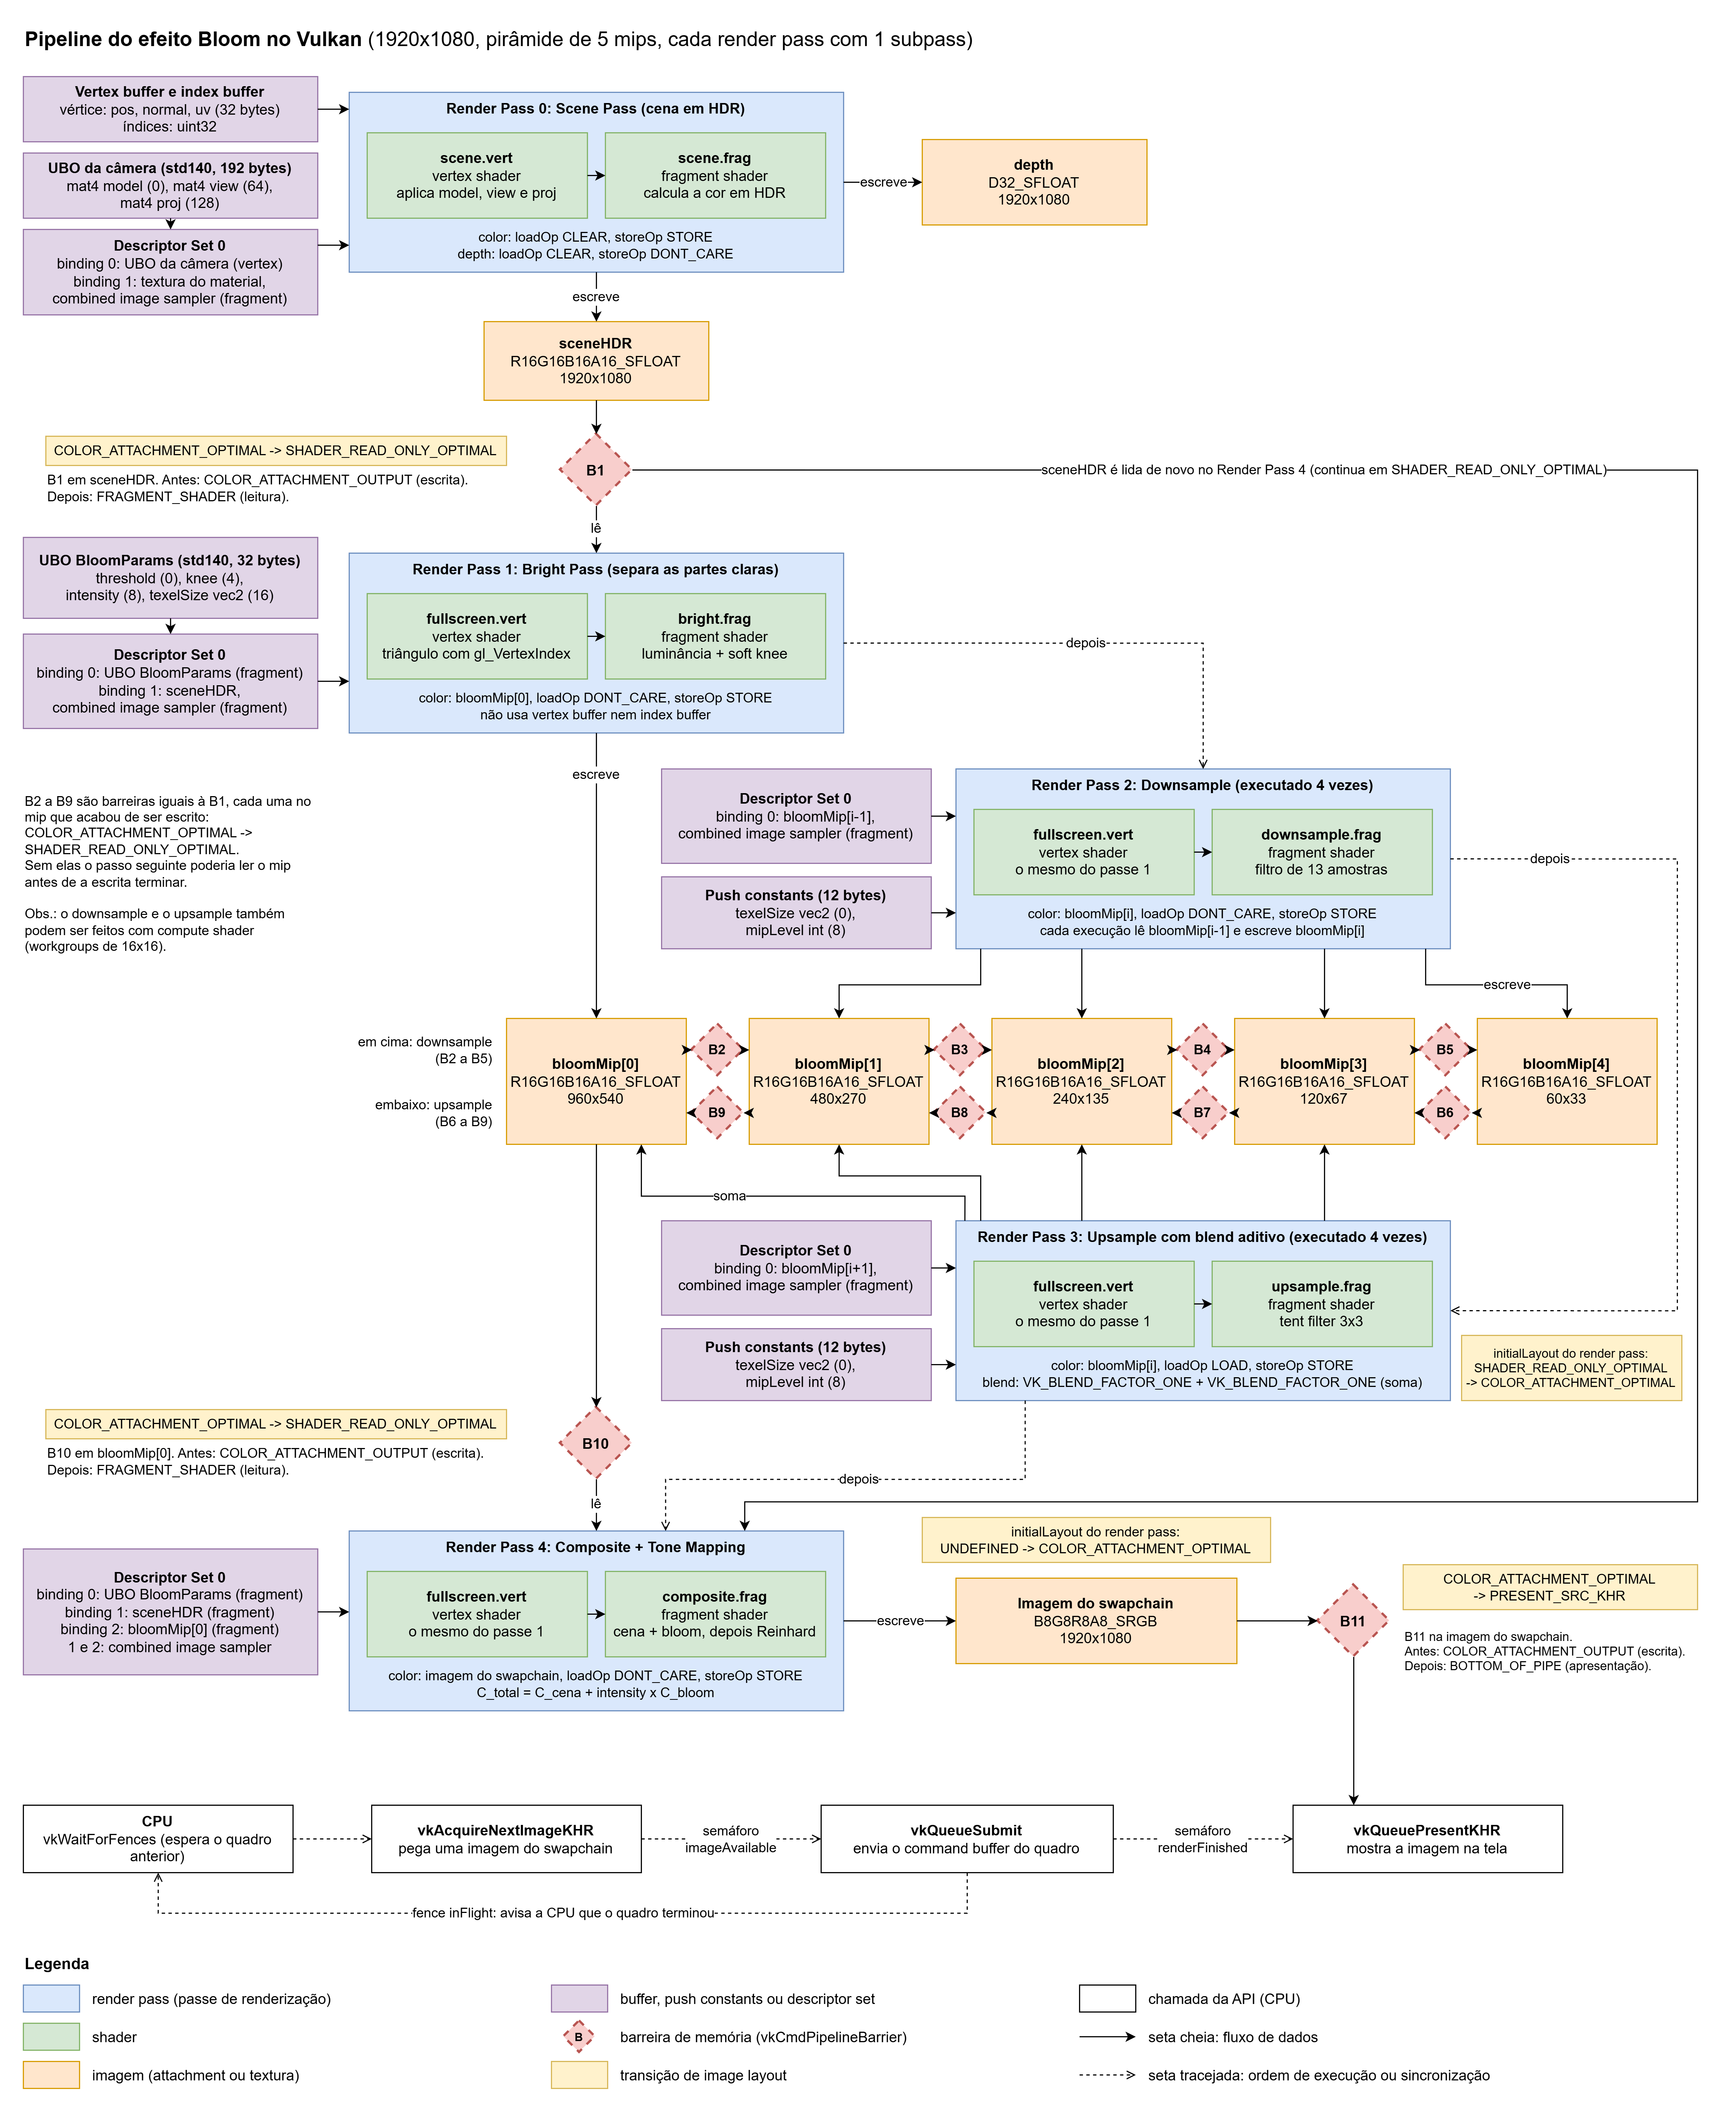
\includegraphics[height=0.64\textheight]{diagrama.png}
    \caption{Arquitetura do pipeline Vulkan para o efeito de \textit{Bloom}. Azul: \textit{render pass}. Verde: \textit{shader}. Laranja: imagem. Roxo: \textit{buffer} ou \textit{descriptor set}. Losango vermelho: barreira de memória. Amarelo: transição de \textit{layout}. Seta cheia: dados. Seta tracejada: ordem de execução ou sincronização.}
    \label{fig:pipeline}
\end{figure}

\subsection{Fluxo de Dados}
O quadro é desenhado em onze passes, gravados em ordem em um único \textit{command buffer}:
\begin{enumerate}
    \setlength{\itemsep}{0pt}
    \item \textbf{Passe 0 (\textit{Scene Pass}):} recebe o \textit{vertex buffer}, o \textit{index buffer}, o UBO da câmera e as texturas. Desenha a cena na \texttt{sceneHDR}, usando a \texttt{depth} no teste de profundidade.
    \item \textbf{Passe 1 (\textit{Bright Pass}):} lê a \texttt{sceneHDR} e guarda só as partes claras na \texttt{bloomMip[0]}, com metade da resolução.
    \item \textbf{Passes 2 a 5 (\textit{Downsample}):} cada execução lê \texttt{bloomMip[i-1]} e escreve \texttt{bloomMip[i]}, menor e mais borrado.
    \item \textbf{Passes 6 a 9 (\textit{Upsample}):} cada execução lê \texttt{bloomMip[i+1]} e soma o resultado em \texttt{bloomMip[i]}. No fim, a \texttt{bloomMip[0]} tem o halo completo.
    \item \textbf{Passe 10 (\textit{Composite}):} soma a \texttt{sceneHDR} com a \texttt{bloomMip[0]}, aplica o \textit{tone mapping} e escreve na imagem do \textit{swapchain}, que é mostrada na tela.
\end{enumerate}
\textbf{Recursos compartilhados.} A \texttt{sceneHDR} é lida nos passes 1 e 10. Os níveis \texttt{bloomMip} são \textit{mip levels} de uma mesma \texttt{VkImage}, usados na descida e na subida. O UBO \texttt{BloomParams} serve aos passes 1 e 10, e o \texttt{fullscreen.vert} e o \texttt{VkSampler} são os mesmos em todos os passes de tela cheia.

\subsection{Render Passes e Subpasses}
São cinco \textit{render passes}, todos com um único \textit{subpass} (Tabela~\ref{tab:renderpasses}).

\begin{table}[H]
    \centering
    \caption{\textit{Render passes} do pipeline.}
    \label{tab:renderpasses}
    \vspace{4pt}
    \scriptsize
    \setlength{\tabcolsep}{4pt}
    \begin{tabular}{c c l l l l}
        \toprule
        \textbf{RP} & \textbf{Passes} & \textbf{Attachment} & \textbf{loadOp / storeOp} & \textbf{initialLayout} & \textbf{Resultado} \\
        \midrule
        0 & 0 & \texttt{sceneHDR} (cor) & \texttt{CLEAR / STORE} & \texttt{UNDEFINED} & cena em HDR \\
          &   & \texttt{depth} (profundidade) & \texttt{CLEAR / DONT\_CARE} & \texttt{UNDEFINED} & teste de profundidade \\
        1 & 1 & \texttt{bloomMip[0]} & \texttt{DONT\_CARE / STORE} & \texttt{UNDEFINED} & partes claras da cena \\
        2 & 2 a 5 & \texttt{bloomMip[1]} a \texttt{bloomMip[4]} & \texttt{DONT\_CARE / STORE} & \texttt{UNDEFINED} & nível menor e borrado \\
        3 & 6 a 9 & \texttt{bloomMip[3]} a \texttt{bloomMip[0]} & \texttt{LOAD / STORE} & \texttt{SHADER\_READ\_ONLY\_OPTIMAL} & soma dos níveis \\
        4 & 10 & imagem do \textit{swapchain} & \texttt{DONT\_CARE / STORE} & \texttt{UNDEFINED} & imagem final \\
        \bottomrule
    \end{tabular}
\end{table}

No início do \textit{subpass}, o \textit{render pass} leva o \textit{attachment} do \texttt{initialLayout} para \texttt{COLOR\_ATTACHMENT\_OPTIMAL}. O \textit{upsample} usa \texttt{LOAD} porque precisa manter o conteúdo anterior para a soma. Os passes ficaram em \textit{render passes} separados porque cada um escreve em uma imagem de tamanho diferente e lê \textit{texels} vizinhos da anterior com um \textit{sampler}, o que um \textit{input attachment} não permite. O \texttt{VK\_KHR\_dynamic\_rendering} não foi usado por não ser o modelo visto na disciplina.

\subsection{Descriptor Sets e Bindings}
Todos os pipelines usam só o \textit{set} 0 (Tabela~\ref{tab:descriptors}). No \textit{downsample} e no \textit{upsample} há um \textit{descriptor set} para cada nível lido.

\begin{table}[H]
    \centering
    \caption{\textit{Descriptor sets} e \textit{bindings} de cada passe.}
    \label{tab:descriptors}
    \vspace{4pt}
    \scriptsize
    \setlength{\tabcolsep}{5pt}
    \begin{tabular}{l c c l l l}
        \toprule
        \textbf{Passe} & \textbf{Set} & \textbf{Binding} & \textbf{Tipo} & \textbf{Recurso} & \textbf{Estágio} \\
        \midrule
        0 (\textit{Scene}) & 0 & 0 & \texttt{UNIFORM\_BUFFER} & UBO da câmera & \textit{vertex} \\
                           & 0 & 1 & \texttt{COMBINED\_IMAGE\_SAMPLER} & textura do material & \textit{fragment} \\
        1 (\textit{Bright}) & 0 & 0 & \texttt{UNIFORM\_BUFFER} & \texttt{BloomParams} & \textit{fragment} \\
                            & 0 & 1 & \texttt{COMBINED\_IMAGE\_SAMPLER} & \texttt{sceneHDR} & \textit{fragment} \\
        2 a 5 (\textit{Downsample}) & 0 & 0 & \texttt{COMBINED\_IMAGE\_SAMPLER} & \texttt{bloomMip[i-1]} & \textit{fragment} \\
        6 a 9 (\textit{Upsample}) & 0 & 0 & \texttt{COMBINED\_IMAGE\_SAMPLER} & \texttt{bloomMip[i+1]} & \textit{fragment} \\
        10 (\textit{Composite}) & 0 & 0 & \texttt{UNIFORM\_BUFFER} & \texttt{BloomParams} & \textit{fragment} \\
                                & 0 & 1 & \texttt{COMBINED\_IMAGE\_SAMPLER} & \texttt{sceneHDR} & \textit{fragment} \\
                                & 0 & 2 & \texttt{COMBINED\_IMAGE\_SAMPLER} & \texttt{bloomMip[0]} & \textit{fragment} \\
        \bottomrule
    \end{tabular}
\end{table}

\subsection{Layout e Finalidade dos Buffers}
\begin{itemize}
    \setlength{\itemsep}{0pt}
    \item \textbf{\textit{Vertex buffer} e \textit{index buffer}:} geometria da cena, só no passe 0. Cada vértice tem 32 bytes: posição (\textit{offset} 0), normal (12) e coordenada de textura (24). Os índices são \texttt{uint32}.
    \item \textbf{UBO da câmera} (\texttt{std140}, 192 bytes): matrizes \texttt{model} (0), \texttt{view} (64) e \texttt{proj} (128).
    \item \textbf{UBO \texttt{BloomParams}} (\texttt{std140}, 32 bytes): \texttt{threshold} (0), \texttt{knee} (4), \texttt{intensity} (8) e \texttt{texelSize} (16), que são os parâmetros das Equações~\ref{eq:softknee} e~\ref{eq:reinhard}.
    \item \textbf{\textit{Push constants}} (12 bytes): \texttt{texelSize} (0) e \texttt{mipLevel} (8), que mudam a cada execução do \textit{downsample} e do \textit{upsample}.
\end{itemize}
Os passes 1 a 10 não têm \textit{vertex buffer}: o \texttt{fullscreen.vert} gera o triângulo de tela cheia a partir do \texttt{gl\_VertexIndex}, desenhado com \texttt{vkCmdDraw(3, 1, 0, 0)}.

\subsection{Shaders Envolvidos}
O pipeline usa apenas \textit{vertex} e \textit{fragment shaders}:
\begin{itemize}
    \setlength{\itemsep}{0pt}
    \item \texttt{scene.vert} e \texttt{scene.frag}: transformam os vértices e calculam a cor em HDR, que pode passar de $1.0$. Nos passes 1 a 10 o \textit{vertex shader} é sempre o \texttt{fullscreen.vert}.
    \item \texttt{bright.frag}: luminância (Equação~\ref{eq:luminancia}) e corte com joelho suave (Equação~\ref{eq:softknee}).
    \item \texttt{downsample.frag}: média de 13 amostras que reduz e borra, no papel do filtro da Equação~\ref{eq:gauss}.
    \item \texttt{upsample.frag}: \textit{tent filter} $3 \times 3$. A soma é feita pelo \textit{blend} aditivo, com \texttt{VK\_BLEND\_FACTOR\_ONE} na origem e no destino.
    \item \texttt{composite.frag}: soma a cena com o \textit{Bloom} e aplica o \textit{tone mapping} de Reinhard (Equação~\ref{eq:reinhard}) \cite{reinhard2002tone}.
\end{itemize}

\subsection{Barreiras de Memória e Transições de Layout}
\label{sec:barreiras}
A GPU pode começar a ler uma imagem antes de a escrita terminar. Além disso, o \textit{attachment} fica em \texttt{COLOR\_ATTACHMENT\_OPTIMAL} e a leitura por \textit{sampler} exige \texttt{SHADER\_READ\_ONLY\_OPTIMAL}. Por isso há uma barreira (\texttt{vkCmdPipelineBarrier}) sempre que uma imagem escrita em um passe é lida no seguinte (Tabela~\ref{tab:barreiras}).

\begin{table}[H]
    \centering
    \caption{As 11 barreiras de memória do diagrama.}
    \label{tab:barreiras}
    \vspace{4pt}
    \scriptsize
    \begin{tabular}{l l l @{\hspace{0.9cm}} l l l}
        \toprule
        & \textbf{Imagem} & \textbf{Escrita $\to$ leitura} & & \textbf{Imagem} & \textbf{Escrita $\to$ leitura} \\
        \midrule
        B1 & \texttt{sceneHDR} & passe 0 $\to$ passes 1 e 10 & B7 & \texttt{bloomMip[3]} & passe 6 $\to$ passe 7 \\
        B2 & \texttt{bloomMip[0]} & passe 1 $\to$ passe 2 & B8 & \texttt{bloomMip[2]} & passe 7 $\to$ passe 8 \\
        B3 & \texttt{bloomMip[1]} & passe 2 $\to$ passe 3 & B9 & \texttt{bloomMip[1]} & passe 8 $\to$ passe 9 \\
        B4 & \texttt{bloomMip[2]} & passe 3 $\to$ passe 4 & B10 & \texttt{bloomMip[0]} & passe 9 $\to$ passe 10 \\
        B5 & \texttt{bloomMip[3]} & passe 4 $\to$ passe 5 & B11 & \textit{swapchain} & passe 10 $\to$ apresentação \\
        B6 & \texttt{bloomMip[4]} & passe 5 $\to$ passe 6 & & & \\
        \bottomrule
    \end{tabular}
\end{table}

Nas barreiras B1 a B10 os dados são os mesmos: o acesso anterior é uma escrita (\texttt{COLOR\_ATTACHMENT\_WRITE}) no estágio \texttt{COLOR\_ATTACHMENT\_OUTPUT}, o acesso posterior é uma leitura (\texttt{SHADER\_READ}) no estágio \texttt{FRAGMENT\_SHADER} e o \textit{layout} muda de \texttt{COLOR\_ATTACHMENT\_OPTIMAL} para \texttt{SHADER\_READ\_ONLY\_OPTIMAL}. Na B11 o acesso anterior é o mesmo, depois não há outro acesso da GPU (estágio \texttt{BOTTOM\_OF\_PIPE}) e o \textit{layout} vira \texttt{PRESENT\_SRC\_KHR}, exigido para a apresentação. O motivo é igual em todas: a imagem só pode ser usada depois que a escrita terminou e ela está no \textit{layout} certo.

As outras transições de \textit{layout} são feitas pelos \textit{render passes} com o \texttt{initialLayout} e aparecem em amarelo no diagrama. A \texttt{sceneHDR} é lida de novo no passe 10 sem outra barreira, porque continua no \textit{layout} de leitura. A sincronização entre CPU e GPU usa os semáforos \texttt{imageAvailable} e \texttt{renderFinished} e a \textit{fence} \texttt{inFlight}, mostrados na parte de baixo do diagrama.

\subsection{Justificativa das Decisões}
\begin{itemize}
    \setlength{\itemsep}{0pt}
    \item \textbf{Triângulo de tela cheia:} dispensa \textit{vertex buffer} e evita a diagonal que um \textit{quad} teria (Seção~\ref{sec:vulkan}).
    \item \textbf{Pirâmide de \textit{mips}:} um borrão largo feito de uma vez em resolução cheia precisaria de muitas amostras por pixel (Equação~\ref{eq:gauss}). Com a imagem reduzida pela metade a cada nível, um filtro pequeno alcança um raio grande, e a soma dos níveis lembra o espalhamento de Spencer et al. \cite{spencer1995glare}.
    \item \textbf{Formato de 16 bits em ponto flutuante:} guarda valores acima de $1.0$, que diferenciam uma luz forte de uma superfície branca \cite{seetzen2004hdr}. Com 8 bits eles seriam cortados.
    \item \textbf{\textit{Fragment shader} em vez de \textit{compute shader}:} a Seção~\ref{sec:vulkan} cita que o borrão também pode usar \textit{compute shaders} em \textit{workgroups} de $16 \times 16$. O grupo desenhou a versão com \textit{fragment shader} por ser mais simples: todos os passes têm a mesma estrutura e as barreiras são iguais. Com \textit{compute}, o destino seria uma \texttt{STORAGE\_IMAGE} no \textit{layout} \texttt{GENERAL} e as barreiras usariam o estágio \texttt{COMPUTE\_SHADER}.
\end{itemize}
\textbf{Relação com a técnica.} O desenho segue as quatro fases da Seção~\ref{sec:funciona}: \textit{bright pass} (passe 1), \textit{downsampling} (passes 2 a 5), \textit{upsampling} com soma (passes 6 a 9) e composição com \textit{tone mapping} (passe 10). Os recursos também são próprios do \textit{Bloom}: a \texttt{sceneHDR} em ponto flutuante, a pirâmide \texttt{bloomMip}, o \textit{blend} aditivo e o UBO com o limiar e a intensidade.
\fussy

% ===============================================================

\section{Arquitetura do Pipeline Vulkan}
\label{sec:arquitetura}
\sloppy

Esta seção é a segunda entrega do trabalho. A Figura~\ref{fig:pipeline} mostra o desenho do pipeline Vulkan que executa o \textit{Bloom}, feito no draw.io. Como exemplo, o grupo considerou uma tela de $1920 \times 1080$, imagens no formato \texttt{VK\_FORMAT\_R16G16B16A16\_SFLOAT}, citado na Seção~\ref{sec:vulkan}, e uma pirâmide de cinco níveis, de \texttt{bloomMip[0]} a \texttt{bloomMip[4]}.

\begin{figure}[H]
    \centering
    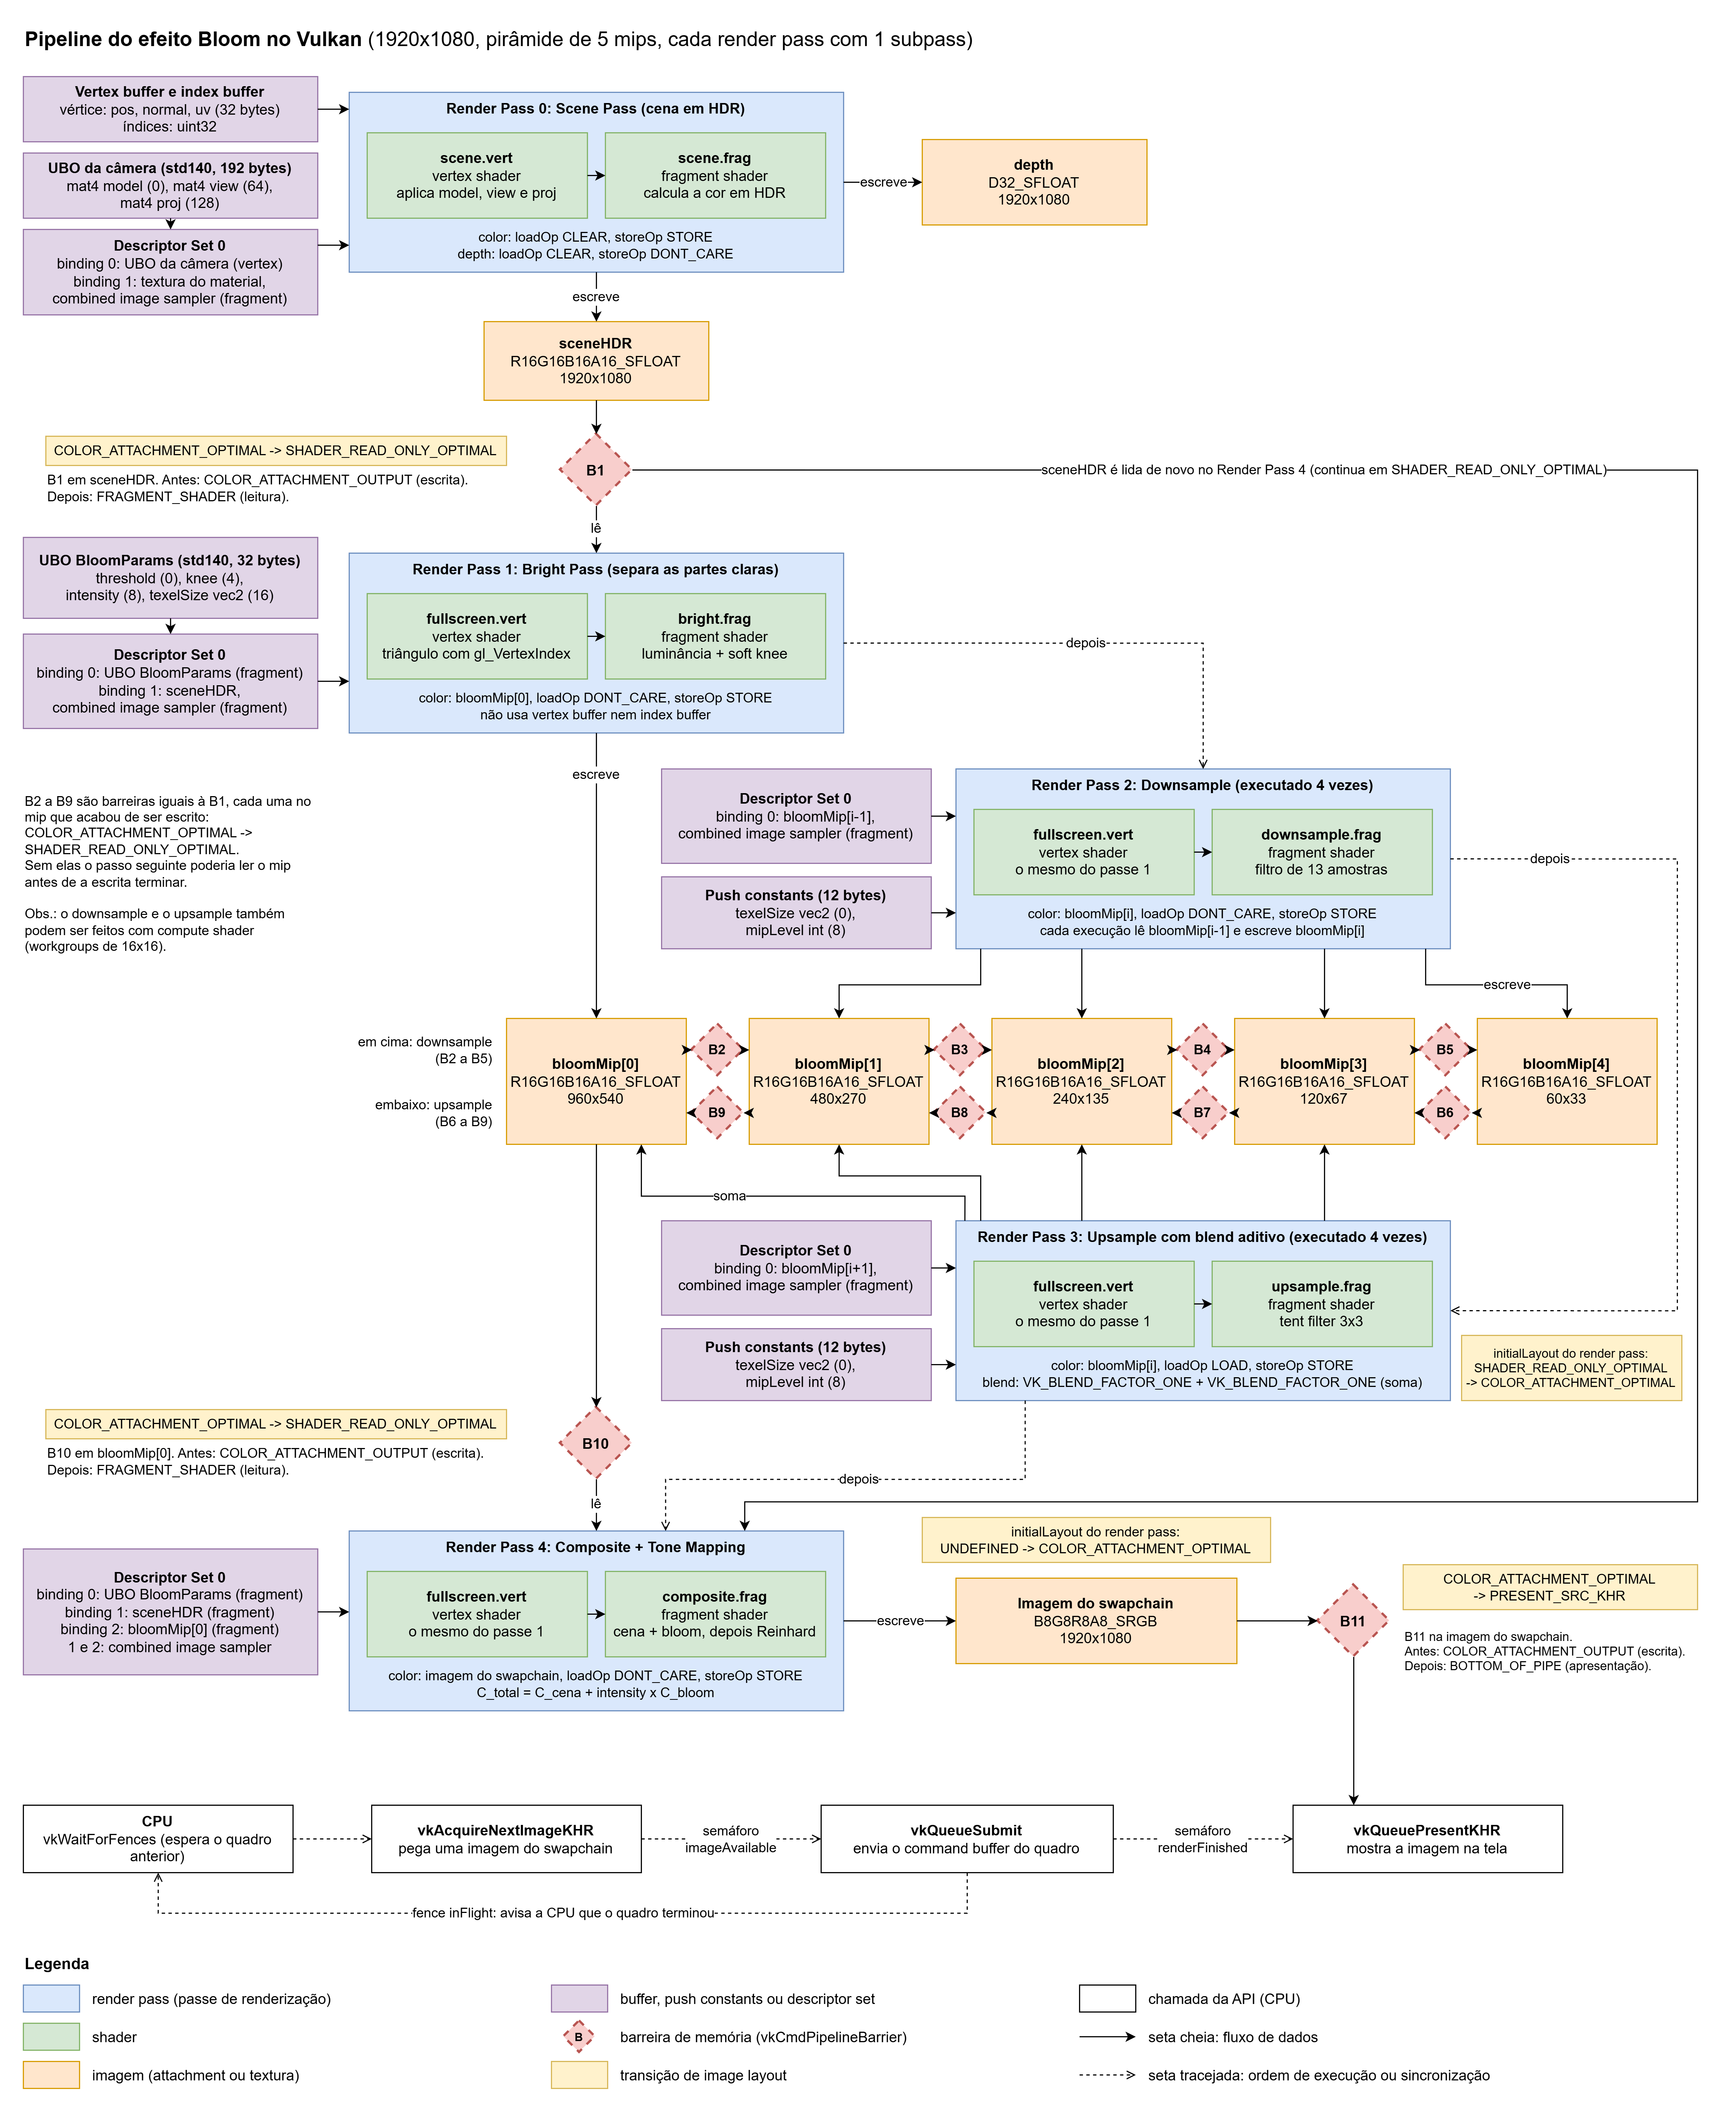
\includegraphics[height=0.64\textheight]{diagrama.png}
    \caption{Arquitetura do pipeline Vulkan para o efeito de \textit{Bloom}. Azul: \textit{render pass}. Verde: \textit{shader}. Laranja: imagem. Roxo: \textit{buffer} ou \textit{descriptor set}. Losango vermelho: barreira de memória. Amarelo: transição de \textit{layout}. Seta cheia: dados. Seta tracejada: ordem de execução ou sincronização.}
    \label{fig:pipeline}
\end{figure}

\subsection{Fluxo de Dados}
O quadro é desenhado em onze passes, gravados em ordem em um único \textit{command buffer}:
\begin{enumerate}
    \setlength{\itemsep}{0pt}
    \item \textbf{Passe 0 (\textit{Scene Pass}):} recebe o \textit{vertex buffer}, o \textit{index buffer}, o UBO da câmera e as texturas. Desenha a cena na \texttt{sceneHDR}, usando a \texttt{depth} no teste de profundidade.
    \item \textbf{Passe 1 (\textit{Bright Pass}):} lê a \texttt{sceneHDR} e guarda só as partes claras na \texttt{bloomMip[0]}, com metade da resolução.
    \item \textbf{Passes 2 a 5 (\textit{Downsample}):} cada execução lê \texttt{bloomMip[i-1]} e escreve \texttt{bloomMip[i]}, menor e mais borrado.
    \item \textbf{Passes 6 a 9 (\textit{Upsample}):} cada execução lê \texttt{bloomMip[i+1]} e soma o resultado em \texttt{bloomMip[i]}. No fim, a \texttt{bloomMip[0]} tem o halo completo.
    \item \textbf{Passe 10 (\textit{Composite}):} soma a \texttt{sceneHDR} com a \texttt{bloomMip[0]}, aplica o \textit{tone mapping} e escreve na imagem do \textit{swapchain}, que é mostrada na tela.
\end{enumerate}
\textbf{Recursos compartilhados.} A \texttt{sceneHDR} é lida nos passes 1 e 10. Os níveis \texttt{bloomMip} são \textit{mip levels} de uma mesma \texttt{VkImage}, usados na descida e na subida. O UBO \texttt{BloomParams} serve aos passes 1 e 10, e o \texttt{fullscreen.vert} e o \texttt{VkSampler} são os mesmos em todos os passes de tela cheia.

\subsection{Render Passes e Subpasses}
São cinco \textit{render passes}, todos com um único \textit{subpass} (Tabela~\ref{tab:renderpasses}).

\begin{table}[H]
    \centering
    \caption{\textit{Render passes} do pipeline.}
    \label{tab:renderpasses}
    \vspace{4pt}
    \scriptsize
    \setlength{\tabcolsep}{4pt}
    \begin{tabular}{c c l l l l}
        \toprule
        \textbf{RP} & \textbf{Passes} & \textbf{Attachment} & \textbf{loadOp / storeOp} & \textbf{initialLayout} & \textbf{Resultado} \\
        \midrule
        0 & 0 & \texttt{sceneHDR} (cor) & \texttt{CLEAR / STORE} & \texttt{UNDEFINED} & cena em HDR \\
          &   & \texttt{depth} (profundidade) & \texttt{CLEAR / DONT\_CARE} & \texttt{UNDEFINED} & teste de profundidade \\
        1 & 1 & \texttt{bloomMip[0]} & \texttt{DONT\_CARE / STORE} & \texttt{UNDEFINED} & partes claras da cena \\
        2 & 2 a 5 & \texttt{bloomMip[1]} a \texttt{bloomMip[4]} & \texttt{DONT\_CARE / STORE} & \texttt{UNDEFINED} & nível menor e borrado \\
        3 & 6 a 9 & \texttt{bloomMip[3]} a \texttt{bloomMip[0]} & \texttt{LOAD / STORE} & \texttt{SHADER\_READ\_ONLY\_OPTIMAL} & soma dos níveis \\
        4 & 10 & imagem do \textit{swapchain} & \texttt{DONT\_CARE / STORE} & \texttt{UNDEFINED} & imagem final \\
        \bottomrule
    \end{tabular}
\end{table}

No início do \textit{subpass}, o \textit{render pass} leva o \textit{attachment} do \texttt{initialLayout} para \texttt{COLOR\_ATTACHMENT\_OPTIMAL}. O \textit{upsample} usa \texttt{LOAD} porque precisa manter o conteúdo anterior para a soma. Os passes ficaram em \textit{render passes} separados porque cada um escreve em uma imagem de tamanho diferente e lê \textit{texels} vizinhos da anterior com um \textit{sampler}, o que um \textit{input attachment} não permite. O \texttt{VK\_KHR\_dynamic\_rendering} não foi usado por não ser o modelo visto na disciplina.

\subsection{Descriptor Sets e Bindings}
Todos os pipelines usam só o \textit{set} 0 (Tabela~\ref{tab:descriptors}). No \textit{downsample} e no \textit{upsample} há um \textit{descriptor set} para cada nível lido.

\begin{table}[H]
    \centering
    \caption{\textit{Descriptor sets} e \textit{bindings} de cada passe.}
    \label{tab:descriptors}
    \vspace{4pt}
    \scriptsize
    \setlength{\tabcolsep}{5pt}
    \begin{tabular}{l c c l l l}
        \toprule
        \textbf{Passe} & \textbf{Set} & \textbf{Binding} & \textbf{Tipo} & \textbf{Recurso} & \textbf{Estágio} \\
        \midrule
        0 (\textit{Scene}) & 0 & 0 & \texttt{UNIFORM\_BUFFER} & UBO da câmera & \textit{vertex} \\
                           & 0 & 1 & \texttt{COMBINED\_IMAGE\_SAMPLER} & textura do material & \textit{fragment} \\
        1 (\textit{Bright}) & 0 & 0 & \texttt{UNIFORM\_BUFFER} & \texttt{BloomParams} & \textit{fragment} \\
                            & 0 & 1 & \texttt{COMBINED\_IMAGE\_SAMPLER} & \texttt{sceneHDR} & \textit{fragment} \\
        2 a 5 (\textit{Downsample}) & 0 & 0 & \texttt{COMBINED\_IMAGE\_SAMPLER} & \texttt{bloomMip[i-1]} & \textit{fragment} \\
        6 a 9 (\textit{Upsample}) & 0 & 0 & \texttt{COMBINED\_IMAGE\_SAMPLER} & \texttt{bloomMip[i+1]} & \textit{fragment} \\
        10 (\textit{Composite}) & 0 & 0 & \texttt{UNIFORM\_BUFFER} & \texttt{BloomParams} & \textit{fragment} \\
                                & 0 & 1 & \texttt{COMBINED\_IMAGE\_SAMPLER} & \texttt{sceneHDR} & \textit{fragment} \\
                                & 0 & 2 & \texttt{COMBINED\_IMAGE\_SAMPLER} & \texttt{bloomMip[0]} & \textit{fragment} \\
        \bottomrule
    \end{tabular}
\end{table}

\subsection{Layout e Finalidade dos Buffers}
\begin{itemize}
    \setlength{\itemsep}{0pt}
    \item \textbf{\textit{Vertex buffer} e \textit{index buffer}:} geometria da cena, só no passe 0. Cada vértice tem 32 bytes: posição (\textit{offset} 0), normal (12) e coordenada de textura (24). Os índices são \texttt{uint32}.
    \item \textbf{UBO da câmera} (\texttt{std140}, 192 bytes): matrizes \texttt{model} (0), \texttt{view} (64) e \texttt{proj} (128).
    \item \textbf{UBO \texttt{BloomParams}} (\texttt{std140}, 32 bytes): \texttt{threshold} (0), \texttt{knee} (4), \texttt{intensity} (8) e \texttt{texelSize} (16), que são os parâmetros das Equações~\ref{eq:softknee} e~\ref{eq:reinhard}.
    \item \textbf{\textit{Push constants}} (12 bytes): \texttt{texelSize} (0) e \texttt{mipLevel} (8), que mudam a cada execução do \textit{downsample} e do \textit{upsample}.
\end{itemize}
Os passes 1 a 10 não têm \textit{vertex buffer}: o \texttt{fullscreen.vert} gera o triângulo de tela cheia a partir do \texttt{gl\_VertexIndex}, desenhado com \texttt{vkCmdDraw(3, 1, 0, 0)}.

\subsection{Shaders Envolvidos}
O pipeline usa apenas \textit{vertex} e \textit{fragment shaders}:
\begin{itemize}
    \setlength{\itemsep}{0pt}
    \item \texttt{scene.vert} e \texttt{scene.frag}: transformam os vértices e calculam a cor em HDR, que pode passar de $1.0$. Nos passes 1 a 10 o \textit{vertex shader} é sempre o \texttt{fullscreen.vert}.
    \item \texttt{bright.frag}: luminância (Equação~\ref{eq:luminancia}) e corte com joelho suave (Equação~\ref{eq:softknee}).
    \item \texttt{downsample.frag}: média de 13 amostras que reduz e borra, no papel do filtro da Equação~\ref{eq:gauss}.
    \item \texttt{upsample.frag}: \textit{tent filter} $3 \times 3$. A soma é feita pelo \textit{blend} aditivo, com \texttt{VK\_BLEND\_FACTOR\_ONE} na origem e no destino.
    \item \texttt{composite.frag}: soma a cena com o \textit{Bloom} e aplica o \textit{tone mapping} de Reinhard (Equação~\ref{eq:reinhard}) \cite{reinhard2002tone}.
\end{itemize}

\subsection{Barreiras de Memória e Transições de Layout}
\label{sec:barreiras}
A GPU pode começar a ler uma imagem antes de a escrita terminar. Além disso, o \textit{attachment} fica em \texttt{COLOR\_ATTACHMENT\_OPTIMAL} e a leitura por \textit{sampler} exige \texttt{SHADER\_READ\_ONLY\_OPTIMAL}. Por isso há uma barreira (\texttt{vkCmdPipelineBarrier}) sempre que uma imagem escrita em um passe é lida no seguinte (Tabela~\ref{tab:barreiras}).

\begin{table}[H]
    \centering
    \caption{As 11 barreiras de memória do diagrama.}
    \label{tab:barreiras}
    \vspace{4pt}
    \scriptsize
    \begin{tabular}{l l l @{\hspace{0.9cm}} l l l}
        \toprule
        & \textbf{Imagem} & \textbf{Escrita $\to$ leitura} & & \textbf{Imagem} & \textbf{Escrita $\to$ leitura} \\
        \midrule
        B1 & \texttt{sceneHDR} & passe 0 $\to$ passes 1 e 10 & B7 & \texttt{bloomMip[3]} & passe 6 $\to$ passe 7 \\
        B2 & \texttt{bloomMip[0]} & passe 1 $\to$ passe 2 & B8 & \texttt{bloomMip[2]} & passe 7 $\to$ passe 8 \\
        B3 & \texttt{bloomMip[1]} & passe 2 $\to$ passe 3 & B9 & \texttt{bloomMip[1]} & passe 8 $\to$ passe 9 \\
        B4 & \texttt{bloomMip[2]} & passe 3 $\to$ passe 4 & B10 & \texttt{bloomMip[0]} & passe 9 $\to$ passe 10 \\
        B5 & \texttt{bloomMip[3]} & passe 4 $\to$ passe 5 & B11 & \textit{swapchain} & passe 10 $\to$ apresentação \\
        B6 & \texttt{bloomMip[4]} & passe 5 $\to$ passe 6 & & & \\
        \bottomrule
    \end{tabular}
\end{table}

Nas barreiras B1 a B10 os dados são os mesmos: o acesso anterior é uma escrita (\texttt{COLOR\_ATTACHMENT\_WRITE}) no estágio \texttt{COLOR\_ATTACHMENT\_OUTPUT}, o acesso posterior é uma leitura (\texttt{SHADER\_READ}) no estágio \texttt{FRAGMENT\_SHADER} e o \textit{layout} muda de \texttt{COLOR\_ATTACHMENT\_OPTIMAL} para \texttt{SHADER\_READ\_ONLY\_OPTIMAL}. Na B11 o acesso anterior é o mesmo, depois não há outro acesso da GPU (estágio \texttt{BOTTOM\_OF\_PIPE}) e o \textit{layout} vira \texttt{PRESENT\_SRC\_KHR}, exigido para a apresentação. O motivo é igual em todas: a imagem só pode ser usada depois que a escrita terminou e ela está no \textit{layout} certo.

As outras transições de \textit{layout} são feitas pelos \textit{render passes} com o \texttt{initialLayout} e aparecem em amarelo no diagrama. A \texttt{sceneHDR} é lida de novo no passe 10 sem outra barreira, porque continua no \textit{layout} de leitura. A sincronização entre CPU e GPU usa os semáforos \texttt{imageAvailable} e \texttt{renderFinished} e a \textit{fence} \texttt{inFlight}, mostrados na parte de baixo do diagrama.

\subsection{Justificativa das Decisões}
\begin{itemize}
    \setlength{\itemsep}{0pt}
    \item \textbf{Triângulo de tela cheia:} dispensa \textit{vertex buffer} e evita a diagonal que um \textit{quad} teria (Seção~\ref{sec:vulkan}).
    \item \textbf{Pirâmide de \textit{mips}:} um borrão largo feito de uma vez em resolução cheia precisaria de muitas amostras por pixel (Equação~\ref{eq:gauss}). Com a imagem reduzida pela metade a cada nível, um filtro pequeno alcança um raio grande, e a soma dos níveis lembra o espalhamento de Spencer et al. \cite{spencer1995glare}.
    \item \textbf{Formato de 16 bits em ponto flutuante:} guarda valores acima de $1.0$, que diferenciam uma luz forte de uma superfície branca \cite{seetzen2004hdr}. Com 8 bits eles seriam cortados.
    \item \textbf{\textit{Fragment shader} em vez de \textit{compute shader}:} a Seção~\ref{sec:vulkan} cita que o borrão também pode usar \textit{compute shaders} em \textit{workgroups} de $16 \times 16$. O grupo desenhou a versão com \textit{fragment shader} por ser mais simples: todos os passes têm a mesma estrutura e as barreiras são iguais. Com \textit{compute}, o destino seria uma \texttt{STORAGE\_IMAGE} no \textit{layout} \texttt{GENERAL} e as barreiras usariam o estágio \texttt{COMPUTE\_SHADER}.
\end{itemize}
\textbf{Relação com a técnica.} O desenho segue as quatro fases da Seção~\ref{sec:funciona}: \textit{bright pass} (passe 1), \textit{downsampling} (passes 2 a 5), \textit{upsampling} com soma (passes 6 a 9) e composição com \textit{tone mapping} (passe 10). Os recursos também são próprios do \textit{Bloom}: a \texttt{sceneHDR} em ponto flutuante, a pirâmide \texttt{bloomMip}, o \textit{blend} aditivo e o UBO com o limiar e a intensidade.
\fussy

% ===============================================================

\section{Arquitetura do Pipeline Vulkan}
\label{sec:arquitetura}
\sloppy

Esta seção é a segunda entrega do trabalho. A Figura~\ref{fig:pipeline} mostra o desenho do pipeline Vulkan que executa o \textit{Bloom}, feito no draw.io. Como exemplo, o grupo considerou uma tela de $1920 \times 1080$, imagens no formato \texttt{VK\_FORMAT\_R16G16B16A16\_SFLOAT}, citado na Seção~\ref{sec:vulkan}, e uma pirâmide de cinco níveis, de \texttt{bloomMip[0]} a \texttt{bloomMip[4]}.

\begin{figure}[H]
    \centering
    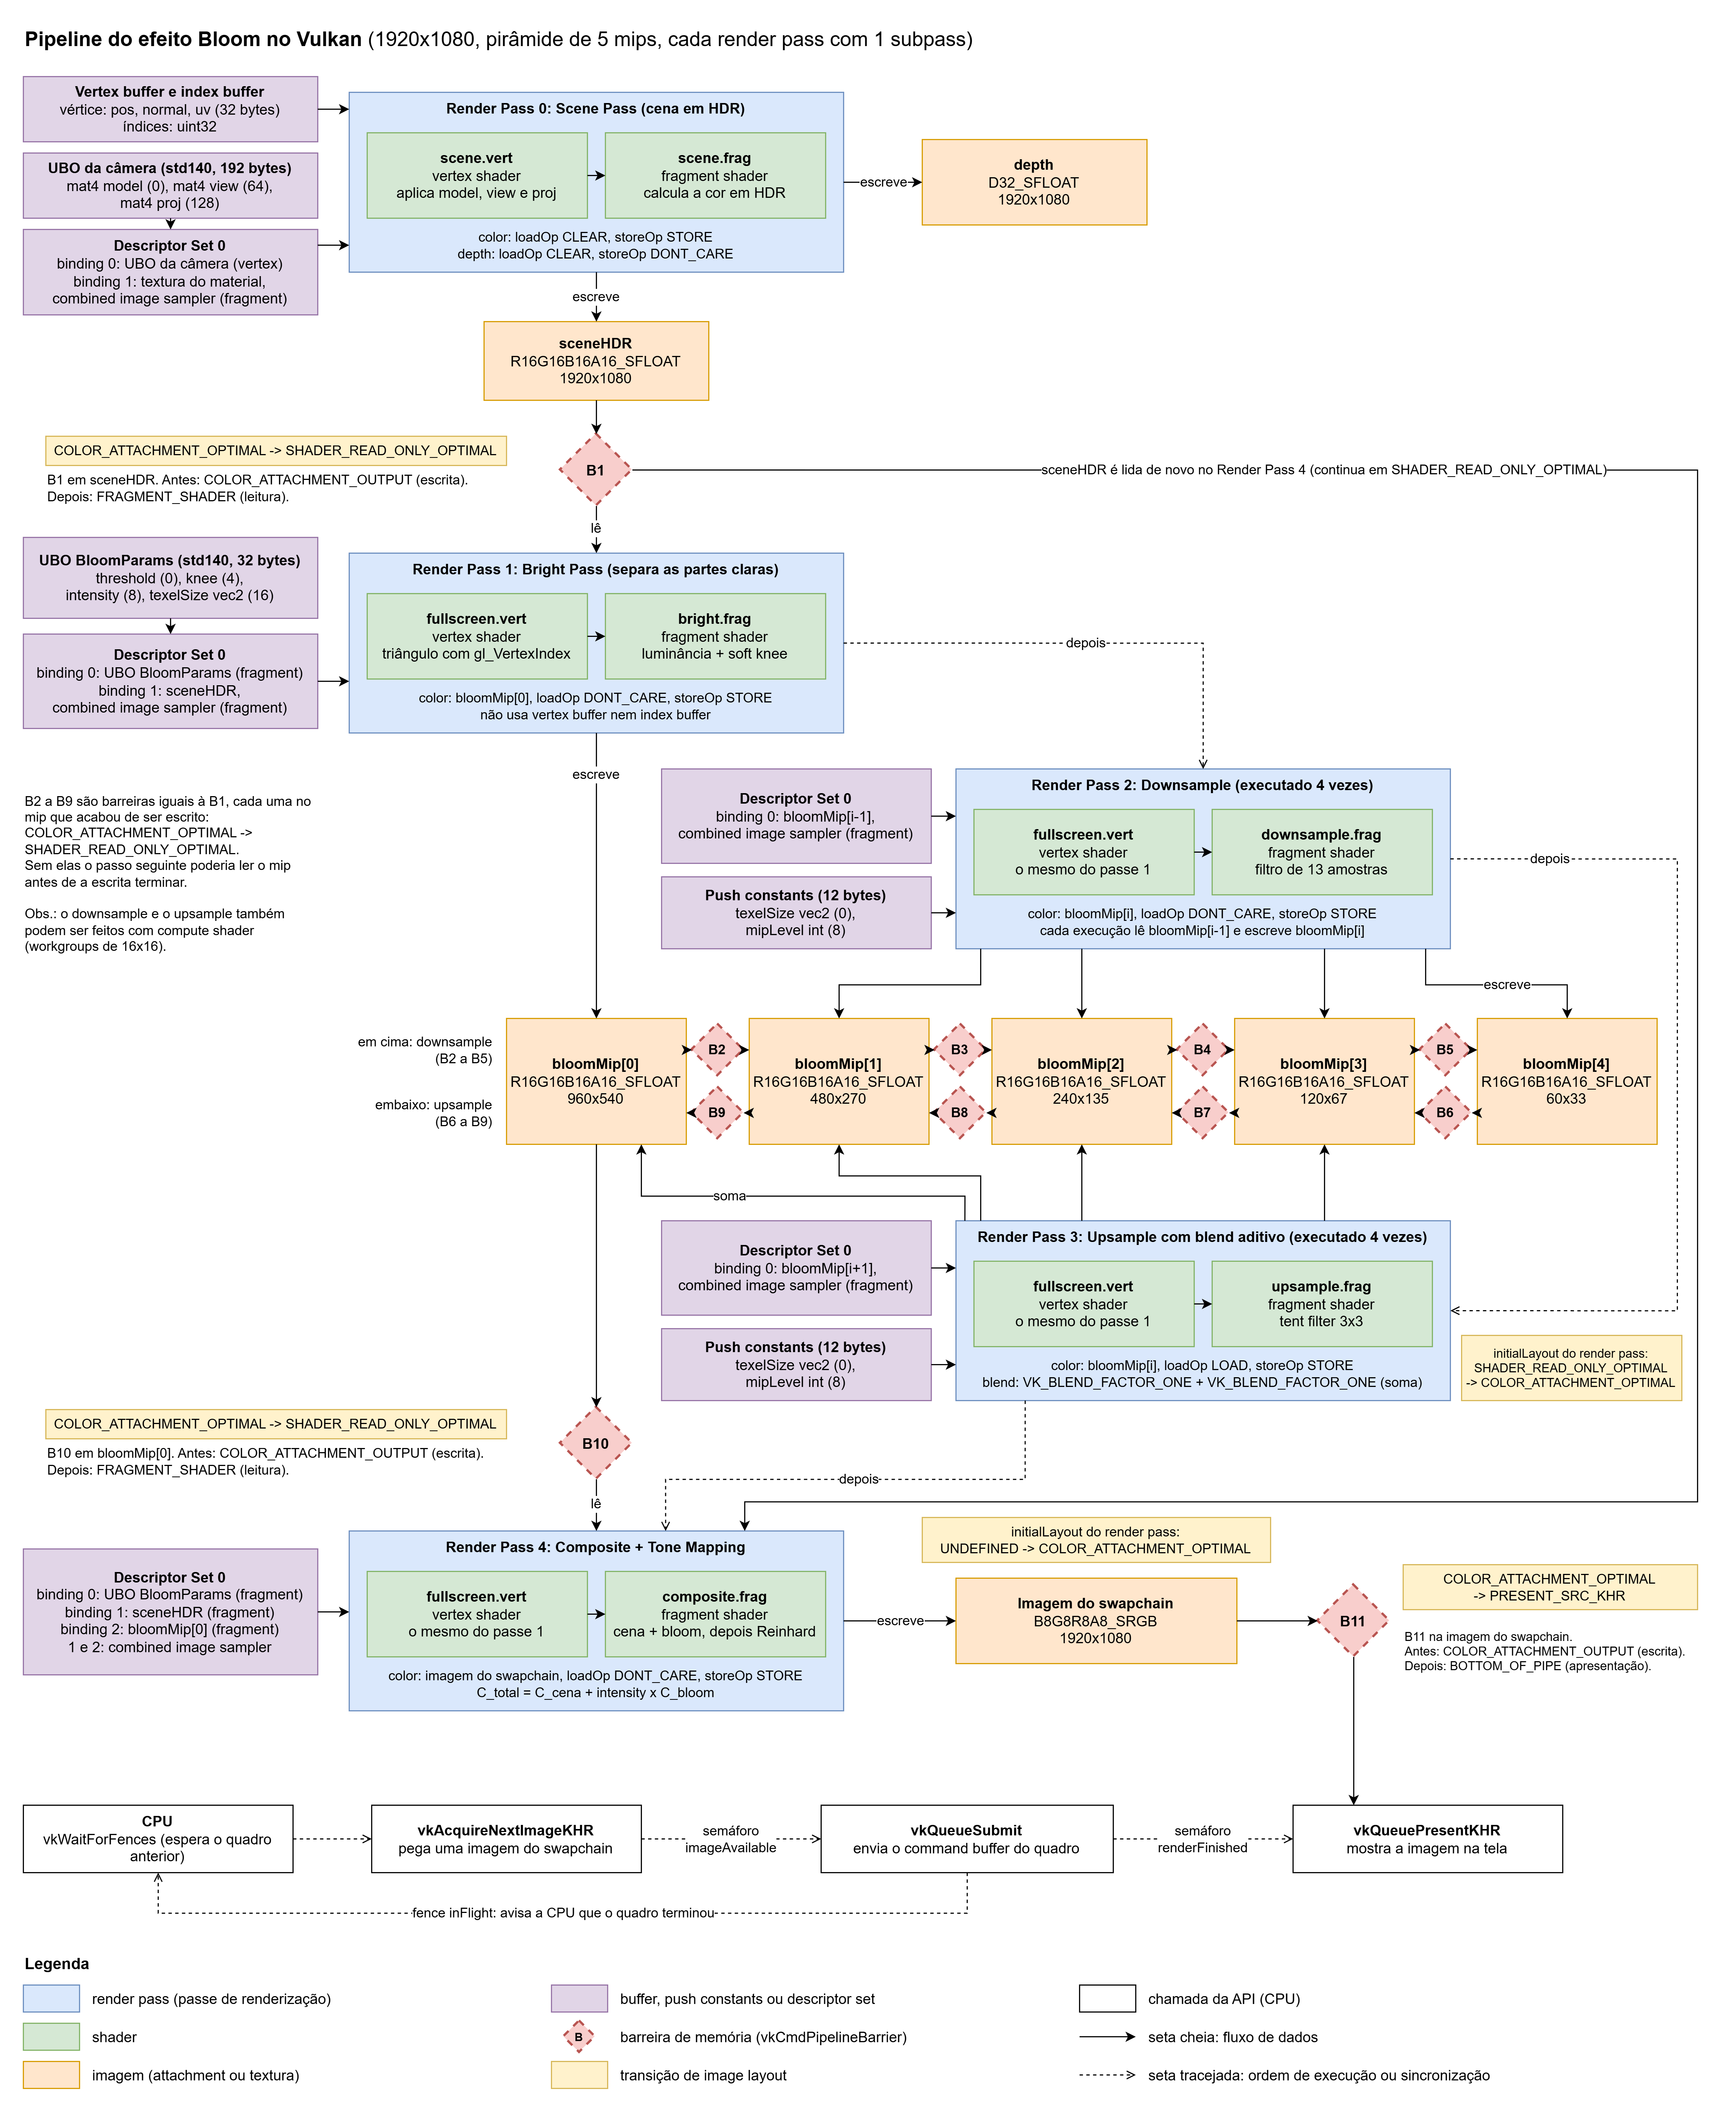
\includegraphics[height=0.64\textheight]{diagrama.png}
    \caption{Arquitetura do pipeline Vulkan para o efeito de \textit{Bloom}. Azul: \textit{render pass}. Verde: \textit{shader}. Laranja: imagem. Roxo: \textit{buffer} ou \textit{descriptor set}. Losango vermelho: barreira de memória. Amarelo: transição de \textit{layout}. Seta cheia: dados. Seta tracejada: ordem de execução ou sincronização.}
    \label{fig:pipeline}
\end{figure}

\subsection{Fluxo de Dados}
O quadro é desenhado em onze passes, gravados em ordem em um único \textit{command buffer}:
\begin{enumerate}
    \setlength{\itemsep}{0pt}
    \item \textbf{Passe 0 (\textit{Scene Pass}):} recebe o \textit{vertex buffer}, o \textit{index buffer}, o UBO da câmera e as texturas. Desenha a cena na \texttt{sceneHDR}, usando a \texttt{depth} no teste de profundidade.
    \item \textbf{Passe 1 (\textit{Bright Pass}):} lê a \texttt{sceneHDR} e guarda só as partes claras na \texttt{bloomMip[0]}, com metade da resolução.
    \item \textbf{Passes 2 a 5 (\textit{Downsample}):} cada execução lê \texttt{bloomMip[i-1]} e escreve \texttt{bloomMip[i]}, menor e mais borrado.
    \item \textbf{Passes 6 a 9 (\textit{Upsample}):} cada execução lê \texttt{bloomMip[i+1]} e soma o resultado em \texttt{bloomMip[i]}. No fim, a \texttt{bloomMip[0]} tem o halo completo.
    \item \textbf{Passe 10 (\textit{Composite}):} soma a \texttt{sceneHDR} com a \texttt{bloomMip[0]}, aplica o \textit{tone mapping} e escreve na imagem do \textit{swapchain}, que é mostrada na tela.
\end{enumerate}
\textbf{Recursos compartilhados.} A \texttt{sceneHDR} é lida nos passes 1 e 10. Os níveis \texttt{bloomMip} são \textit{mip levels} de uma mesma \texttt{VkImage}, usados na descida e na subida. O UBO \texttt{BloomParams} serve aos passes 1 e 10, e o \texttt{fullscreen.vert} e o \texttt{VkSampler} são os mesmos em todos os passes de tela cheia.

\subsection{Render Passes e Subpasses}
São cinco \textit{render passes}, todos com um único \textit{subpass} (Tabela~\ref{tab:renderpasses}).

\begin{table}[H]
    \centering
    \caption{\textit{Render passes} do pipeline.}
    \label{tab:renderpasses}
    \vspace{4pt}
    \scriptsize
    \setlength{\tabcolsep}{4pt}
    \begin{tabular}{c c l l l l}
        \toprule
        \textbf{RP} & \textbf{Passes} & \textbf{Attachment} & \textbf{loadOp / storeOp} & \textbf{initialLayout} & \textbf{Resultado} \\
        \midrule
        0 & 0 & \texttt{sceneHDR} (cor) & \texttt{CLEAR / STORE} & \texttt{UNDEFINED} & cena em HDR \\
          &   & \texttt{depth} (profundidade) & \texttt{CLEAR / DONT\_CARE} & \texttt{UNDEFINED} & teste de profundidade \\
        1 & 1 & \texttt{bloomMip[0]} & \texttt{DONT\_CARE / STORE} & \texttt{UNDEFINED} & partes claras da cena \\
        2 & 2 a 5 & \texttt{bloomMip[1]} a \texttt{bloomMip[4]} & \texttt{DONT\_CARE / STORE} & \texttt{UNDEFINED} & nível menor e borrado \\
        3 & 6 a 9 & \texttt{bloomMip[3]} a \texttt{bloomMip[0]} & \texttt{LOAD / STORE} & \texttt{SHADER\_READ\_ONLY\_OPTIMAL} & soma dos níveis \\
        4 & 10 & imagem do \textit{swapchain} & \texttt{DONT\_CARE / STORE} & \texttt{UNDEFINED} & imagem final \\
        \bottomrule
    \end{tabular}
\end{table}

No início do \textit{subpass}, o \textit{render pass} leva o \textit{attachment} do \texttt{initialLayout} para \texttt{COLOR\_ATTACHMENT\_OPTIMAL}. O \textit{upsample} usa \texttt{LOAD} porque precisa manter o conteúdo anterior para a soma. Os passes ficaram em \textit{render passes} separados porque cada um escreve em uma imagem de tamanho diferente e lê \textit{texels} vizinhos da anterior com um \textit{sampler}, o que um \textit{input attachment} não permite. O \texttt{VK\_KHR\_dynamic\_rendering} não foi usado por não ser o modelo visto na disciplina.

\subsection{Descriptor Sets e Bindings}
Todos os pipelines usam só o \textit{set} 0 (Tabela~\ref{tab:descriptors}). No \textit{downsample} e no \textit{upsample} há um \textit{descriptor set} para cada nível lido.

\begin{table}[H]
    \centering
    \caption{\textit{Descriptor sets} e \textit{bindings} de cada passe.}
    \label{tab:descriptors}
    \vspace{4pt}
    \scriptsize
    \setlength{\tabcolsep}{5pt}
    \begin{tabular}{l c c l l l}
        \toprule
        \textbf{Passe} & \textbf{Set} & \textbf{Binding} & \textbf{Tipo} & \textbf{Recurso} & \textbf{Estágio} \\
        \midrule
        0 (\textit{Scene}) & 0 & 0 & \texttt{UNIFORM\_BUFFER} & UBO da câmera & \textit{vertex} \\
                           & 0 & 1 & \texttt{COMBINED\_IMAGE\_SAMPLER} & textura do material & \textit{fragment} \\
        1 (\textit{Bright}) & 0 & 0 & \texttt{UNIFORM\_BUFFER} & \texttt{BloomParams} & \textit{fragment} \\
                            & 0 & 1 & \texttt{COMBINED\_IMAGE\_SAMPLER} & \texttt{sceneHDR} & \textit{fragment} \\
        2 a 5 (\textit{Downsample}) & 0 & 0 & \texttt{COMBINED\_IMAGE\_SAMPLER} & \texttt{bloomMip[i-1]} & \textit{fragment} \\
        6 a 9 (\textit{Upsample}) & 0 & 0 & \texttt{COMBINED\_IMAGE\_SAMPLER} & \texttt{bloomMip[i+1]} & \textit{fragment} \\
        10 (\textit{Composite}) & 0 & 0 & \texttt{UNIFORM\_BUFFER} & \texttt{BloomParams} & \textit{fragment} \\
                                & 0 & 1 & \texttt{COMBINED\_IMAGE\_SAMPLER} & \texttt{sceneHDR} & \textit{fragment} \\
                                & 0 & 2 & \texttt{COMBINED\_IMAGE\_SAMPLER} & \texttt{bloomMip[0]} & \textit{fragment} \\
        \bottomrule
    \end{tabular}
\end{table}

\subsection{Layout e Finalidade dos Buffers}
\begin{itemize}
    \setlength{\itemsep}{0pt}
    \item \textbf{\textit{Vertex buffer} e \textit{index buffer}:} geometria da cena, só no passe 0. Cada vértice tem 32 bytes: posição (\textit{offset} 0), normal (12) e coordenada de textura (24). Os índices são \texttt{uint32}.
    \item \textbf{UBO da câmera} (\texttt{std140}, 192 bytes): matrizes \texttt{model} (0), \texttt{view} (64) e \texttt{proj} (128).
    \item \textbf{UBO \texttt{BloomParams}} (\texttt{std140}, 32 bytes): \texttt{threshold} (0), \texttt{knee} (4), \texttt{intensity} (8) e \texttt{texelSize} (16), que são os parâmetros das Equações~\ref{eq:softknee} e~\ref{eq:reinhard}.
    \item \textbf{\textit{Push constants}} (12 bytes): \texttt{texelSize} (0) e \texttt{mipLevel} (8), que mudam a cada execução do \textit{downsample} e do \textit{upsample}.
\end{itemize}
Os passes 1 a 10 não têm \textit{vertex buffer}: o \texttt{fullscreen.vert} gera o triângulo de tela cheia a partir do \texttt{gl\_VertexIndex}, desenhado com \texttt{vkCmdDraw(3, 1, 0, 0)}.

\subsection{Shaders Envolvidos}
O pipeline usa apenas \textit{vertex} e \textit{fragment shaders}:
\begin{itemize}
    \setlength{\itemsep}{0pt}
    \item \texttt{scene.vert} e \texttt{scene.frag}: transformam os vértices e calculam a cor em HDR, que pode passar de $1.0$. Nos passes 1 a 10 o \textit{vertex shader} é sempre o \texttt{fullscreen.vert}.
    \item \texttt{bright.frag}: luminância (Equação~\ref{eq:luminancia}) e corte com joelho suave (Equação~\ref{eq:softknee}).
    \item \texttt{downsample.frag}: média de 13 amostras que reduz e borra, no papel do filtro da Equação~\ref{eq:gauss}.
    \item \texttt{upsample.frag}: \textit{tent filter} $3 \times 3$. A soma é feita pelo \textit{blend} aditivo, com \texttt{VK\_BLEND\_FACTOR\_ONE} na origem e no destino.
    \item \texttt{composite.frag}: soma a cena com o \textit{Bloom} e aplica o \textit{tone mapping} de Reinhard (Equação~\ref{eq:reinhard}) \cite{reinhard2002tone}.
\end{itemize}

\subsection{Barreiras de Memória e Transições de Layout}
\label{sec:barreiras}
A GPU pode começar a ler uma imagem antes de a escrita terminar. Além disso, o \textit{attachment} fica em \texttt{COLOR\_ATTACHMENT\_OPTIMAL} e a leitura por \textit{sampler} exige \texttt{SHADER\_READ\_ONLY\_OPTIMAL}. Por isso há uma barreira (\texttt{vkCmdPipelineBarrier}) sempre que uma imagem escrita em um passe é lida no seguinte (Tabela~\ref{tab:barreiras}).

\begin{table}[H]
    \centering
    \caption{As 11 barreiras de memória do diagrama.}
    \label{tab:barreiras}
    \vspace{4pt}
    \scriptsize
    \begin{tabular}{l l l @{\hspace{0.9cm}} l l l}
        \toprule
        & \textbf{Imagem} & \textbf{Escrita $\to$ leitura} & & \textbf{Imagem} & \textbf{Escrita $\to$ leitura} \\
        \midrule
        B1 & \texttt{sceneHDR} & passe 0 $\to$ passes 1 e 10 & B7 & \texttt{bloomMip[3]} & passe 6 $\to$ passe 7 \\
        B2 & \texttt{bloomMip[0]} & passe 1 $\to$ passe 2 & B8 & \texttt{bloomMip[2]} & passe 7 $\to$ passe 8 \\
        B3 & \texttt{bloomMip[1]} & passe 2 $\to$ passe 3 & B9 & \texttt{bloomMip[1]} & passe 8 $\to$ passe 9 \\
        B4 & \texttt{bloomMip[2]} & passe 3 $\to$ passe 4 & B10 & \texttt{bloomMip[0]} & passe 9 $\to$ passe 10 \\
        B5 & \texttt{bloomMip[3]} & passe 4 $\to$ passe 5 & B11 & \textit{swapchain} & passe 10 $\to$ apresentação \\
        B6 & \texttt{bloomMip[4]} & passe 5 $\to$ passe 6 & & & \\
        \bottomrule
    \end{tabular}
\end{table}

Nas barreiras B1 a B10 os dados são os mesmos: o acesso anterior é uma escrita (\texttt{COLOR\_ATTACHMENT\_WRITE}) no estágio \texttt{COLOR\_ATTACHMENT\_OUTPUT}, o acesso posterior é uma leitura (\texttt{SHADER\_READ}) no estágio \texttt{FRAGMENT\_SHADER} e o \textit{layout} muda de \texttt{COLOR\_ATTACHMENT\_OPTIMAL} para \texttt{SHADER\_READ\_ONLY\_OPTIMAL}. Na B11 o acesso anterior é o mesmo, depois não há outro acesso da GPU (estágio \texttt{BOTTOM\_OF\_PIPE}) e o \textit{layout} vira \texttt{PRESENT\_SRC\_KHR}, exigido para a apresentação. O motivo é igual em todas: a imagem só pode ser usada depois que a escrita terminou e ela está no \textit{layout} certo.

As outras transições de \textit{layout} são feitas pelos \textit{render passes} com o \texttt{initialLayout} e aparecem em amarelo no diagrama. A \texttt{sceneHDR} é lida de novo no passe 10 sem outra barreira, porque continua no \textit{layout} de leitura. A sincronização entre CPU e GPU usa os semáforos \texttt{imageAvailable} e \texttt{renderFinished} e a \textit{fence} \texttt{inFlight}, mostrados na parte de baixo do diagrama.

\subsection{Justificativa das Decisões}
\begin{itemize}
    \setlength{\itemsep}{0pt}
    \item \textbf{Triângulo de tela cheia:} dispensa \textit{vertex buffer} e evita a diagonal que um \textit{quad} teria (Seção~\ref{sec:vulkan}).
    \item \textbf{Pirâmide de \textit{mips}:} um borrão largo feito de uma vez em resolução cheia precisaria de muitas amostras por pixel (Equação~\ref{eq:gauss}). Com a imagem reduzida pela metade a cada nível, um filtro pequeno alcança um raio grande, e a soma dos níveis lembra o espalhamento de Spencer et al. \cite{spencer1995glare}.
    \item \textbf{Formato de 16 bits em ponto flutuante:} guarda valores acima de $1.0$, que diferenciam uma luz forte de uma superfície branca \cite{seetzen2004hdr}. Com 8 bits eles seriam cortados.
    \item \textbf{\textit{Fragment shader} em vez de \textit{compute shader}:} a Seção~\ref{sec:vulkan} cita que o borrão também pode usar \textit{compute shaders} em \textit{workgroups} de $16 \times 16$. O grupo desenhou a versão com \textit{fragment shader} por ser mais simples: todos os passes têm a mesma estrutura e as barreiras são iguais. Com \textit{compute}, o destino seria uma \texttt{STORAGE\_IMAGE} no \textit{layout} \texttt{GENERAL} e as barreiras usariam o estágio \texttt{COMPUTE\_SHADER}.
\end{itemize}
\textbf{Relação com a técnica.} O desenho segue as quatro fases da Seção~\ref{sec:funciona}: \textit{bright pass} (passe 1), \textit{downsampling} (passes 2 a 5), \textit{upsampling} com soma (passes 6 a 9) e composição com \textit{tone mapping} (passe 10). Os recursos também são próprios do \textit{Bloom}: a \texttt{sceneHDR} em ponto flutuante, a pirâmide \texttt{bloomMip}, o \textit{blend} aditivo e o UBO com o limiar e a intensidade.
\fussy

% ===============================================================

\section{Arquitetura do Pipeline Vulkan}
\label{sec:arquitetura}
\sloppy

Esta seção é a segunda entrega do trabalho. A Figura~\ref{fig:pipeline} mostra o desenho do pipeline Vulkan que executa o \textit{Bloom}, feito no draw.io. Como exemplo, o grupo considerou uma tela de $1920 \times 1080$, imagens no formato \texttt{VK\_FORMAT\_R16G16B16A16\_SFLOAT}, citado na Seção~\ref{sec:vulkan}, e uma pirâmide de cinco níveis, de \texttt{bloomMip[0]} a \texttt{bloomMip[4]}.

\begin{figure}[H]
    \centering
    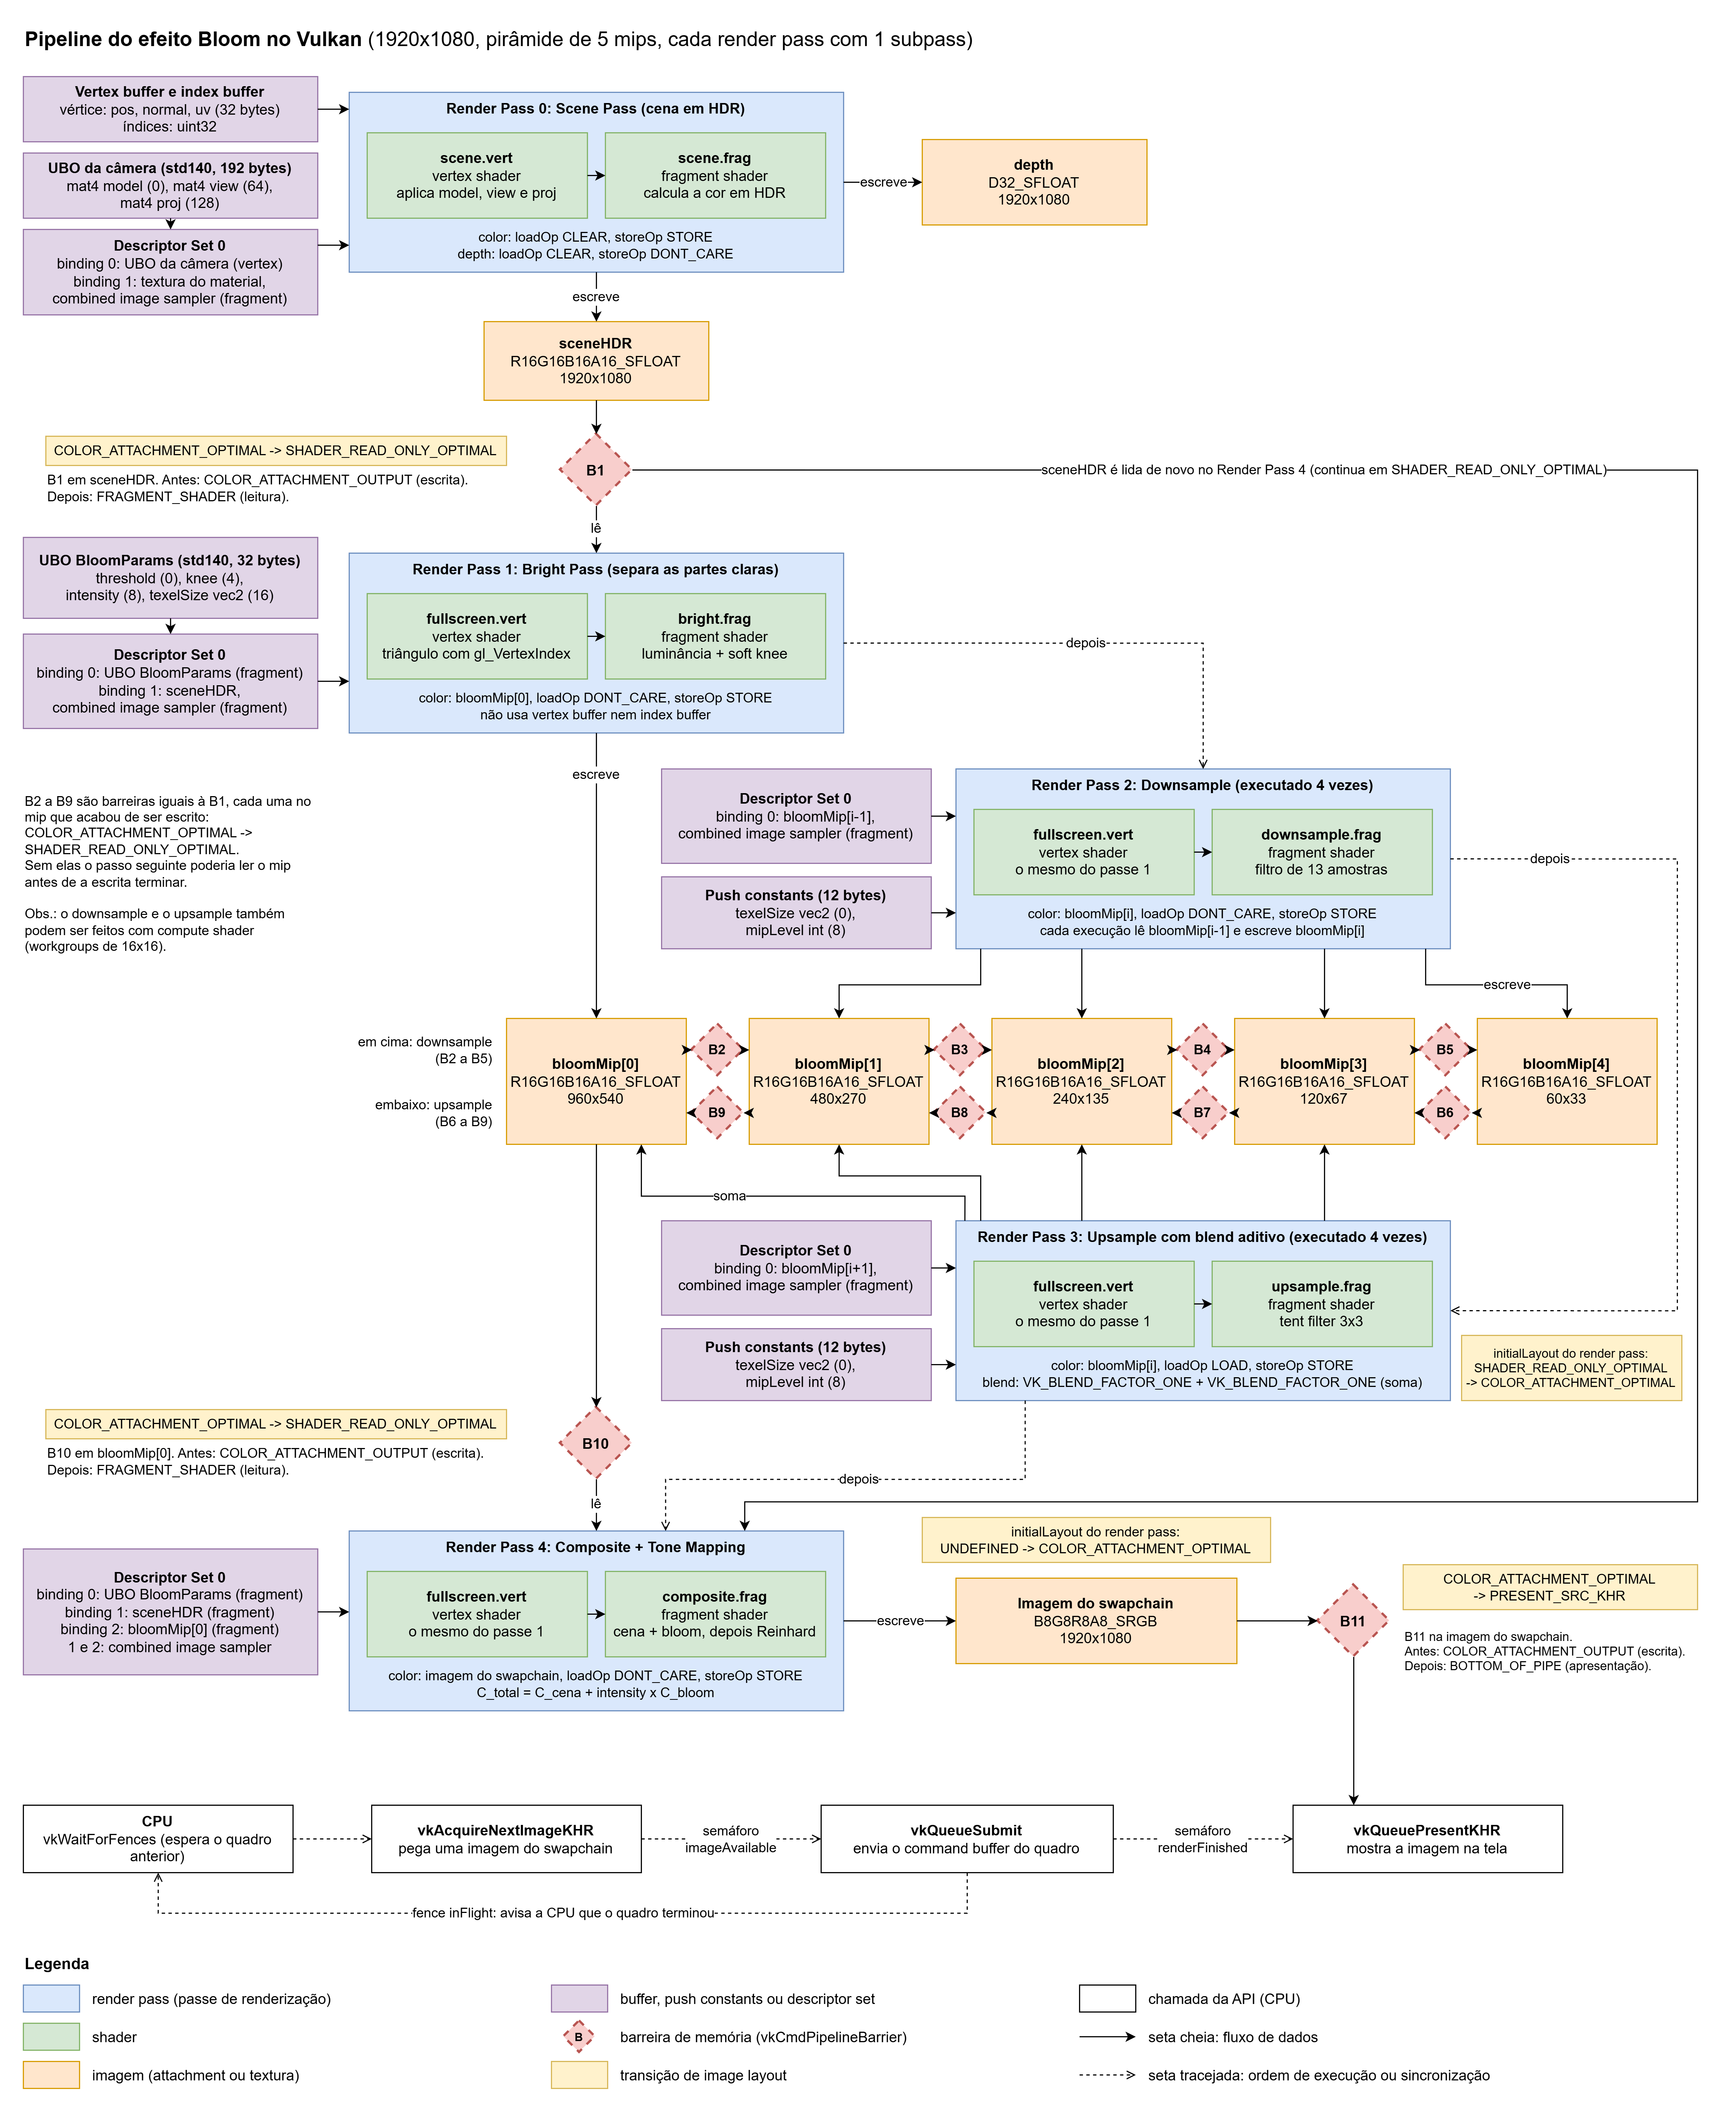
\includegraphics[height=0.64\textheight]{diagrama.png}
    \caption{Arquitetura do pipeline Vulkan para o efeito de \textit{Bloom}. Azul: \textit{render pass}. Verde: \textit{shader}. Laranja: imagem. Roxo: \textit{buffer} ou \textit{descriptor set}. Losango vermelho: barreira de memória. Amarelo: transição de \textit{layout}. Seta cheia: dados. Seta tracejada: ordem de execução ou sincronização.}
    \label{fig:pipeline}
\end{figure}

\subsection{Fluxo de Dados}
O quadro é desenhado em onze passes, gravados em ordem em um único \textit{command buffer}:
\begin{enumerate}
    \setlength{\itemsep}{0pt}
    \item \textbf{Passe 0 (\textit{Scene Pass}):} recebe o \textit{vertex buffer}, o \textit{index buffer}, o UBO da câmera e as texturas. Desenha a cena na \texttt{sceneHDR}, usando a \texttt{depth} no teste de profundidade.
    \item \textbf{Passe 1 (\textit{Bright Pass}):} lê a \texttt{sceneHDR} e guarda só as partes claras na \texttt{bloomMip[0]}, com metade da resolução.
    \item \textbf{Passes 2 a 5 (\textit{Downsample}):} cada execução lê \texttt{bloomMip[i-1]} e escreve \texttt{bloomMip[i]}, menor e mais borrado.
    \item \textbf{Passes 6 a 9 (\textit{Upsample}):} cada execução lê \texttt{bloomMip[i+1]} e soma o resultado em \texttt{bloomMip[i]}. No fim, a \texttt{bloomMip[0]} tem o halo completo.
    \item \textbf{Passe 10 (\textit{Composite}):} soma a \texttt{sceneHDR} com a \texttt{bloomMip[0]}, aplica o \textit{tone mapping} e escreve na imagem do \textit{swapchain}, que é mostrada na tela.
\end{enumerate}
\textbf{Recursos compartilhados.} A \texttt{sceneHDR} é lida nos passes 1 e 10. Os níveis \texttt{bloomMip} são \textit{mip levels} de uma mesma \texttt{VkImage}, usados na descida e na subida. O UBO \texttt{BloomParams} serve aos passes 1 e 10, e o \texttt{fullscreen.vert} e o \texttt{VkSampler} são os mesmos em todos os passes de tela cheia.

\subsection{Render Passes e Subpasses}
São cinco \textit{render passes}, todos com um único \textit{subpass} (Tabela~\ref{tab:renderpasses}).

\begin{table}[H]
    \centering
    \caption{\textit{Render passes} do pipeline.}
    \label{tab:renderpasses}
    \vspace{4pt}
    \scriptsize
    \setlength{\tabcolsep}{4pt}
    \begin{tabular}{c c l l l l}
        \toprule
        \textbf{RP} & \textbf{Passes} & \textbf{Attachment} & \textbf{loadOp / storeOp} & \textbf{initialLayout} & \textbf{Resultado} \\
        \midrule
        0 & 0 & \texttt{sceneHDR} (cor) & \texttt{CLEAR / STORE} & \texttt{UNDEFINED} & cena em HDR \\
          &   & \texttt{depth} (profundidade) & \texttt{CLEAR / DONT\_CARE} & \texttt{UNDEFINED} & teste de profundidade \\
        1 & 1 & \texttt{bloomMip[0]} & \texttt{DONT\_CARE / STORE} & \texttt{UNDEFINED} & partes claras da cena \\
        2 & 2 a 5 & \texttt{bloomMip[1]} a \texttt{bloomMip[4]} & \texttt{DONT\_CARE / STORE} & \texttt{UNDEFINED} & nível menor e borrado \\
        3 & 6 a 9 & \texttt{bloomMip[3]} a \texttt{bloomMip[0]} & \texttt{LOAD / STORE} & \texttt{SHADER\_READ\_ONLY\_OPTIMAL} & soma dos níveis \\
        4 & 10 & imagem do \textit{swapchain} & \texttt{DONT\_CARE / STORE} & \texttt{UNDEFINED} & imagem final \\
        \bottomrule
    \end{tabular}
\end{table}

No início do \textit{subpass}, o \textit{render pass} leva o \textit{attachment} do \texttt{initialLayout} para \texttt{COLOR\_ATTACHMENT\_OPTIMAL}. O \textit{upsample} usa \texttt{LOAD} porque precisa manter o conteúdo anterior para a soma. Os passes ficaram em \textit{render passes} separados porque cada um escreve em uma imagem de tamanho diferente e lê \textit{texels} vizinhos da anterior com um \textit{sampler}, o que um \textit{input attachment} não permite. O \texttt{VK\_KHR\_dynamic\_rendering} não foi usado por não ser o modelo visto na disciplina.

\subsection{Descriptor Sets e Bindings}
Todos os pipelines usam só o \textit{set} 0 (Tabela~\ref{tab:descriptors}). No \textit{downsample} e no \textit{upsample} há um \textit{descriptor set} para cada nível lido.

\begin{table}[H]
    \centering
    \caption{\textit{Descriptor sets} e \textit{bindings} de cada passe.}
    \label{tab:descriptors}
    \vspace{4pt}
    \scriptsize
    \setlength{\tabcolsep}{5pt}
    \begin{tabular}{l c c l l l}
        \toprule
        \textbf{Passe} & \textbf{Set} & \textbf{Binding} & \textbf{Tipo} & \textbf{Recurso} & \textbf{Estágio} \\
        \midrule
        0 (\textit{Scene}) & 0 & 0 & \texttt{UNIFORM\_BUFFER} & UBO da câmera & \textit{vertex} \\
                           & 0 & 1 & \texttt{COMBINED\_IMAGE\_SAMPLER} & textura do material & \textit{fragment} \\
        1 (\textit{Bright}) & 0 & 0 & \texttt{UNIFORM\_BUFFER} & \texttt{BloomParams} & \textit{fragment} \\
                            & 0 & 1 & \texttt{COMBINED\_IMAGE\_SAMPLER} & \texttt{sceneHDR} & \textit{fragment} \\
        2 a 5 (\textit{Downsample}) & 0 & 0 & \texttt{COMBINED\_IMAGE\_SAMPLER} & \texttt{bloomMip[i-1]} & \textit{fragment} \\
        6 a 9 (\textit{Upsample}) & 0 & 0 & \texttt{COMBINED\_IMAGE\_SAMPLER} & \texttt{bloomMip[i+1]} & \textit{fragment} \\
        10 (\textit{Composite}) & 0 & 0 & \texttt{UNIFORM\_BUFFER} & \texttt{BloomParams} & \textit{fragment} \\
                                & 0 & 1 & \texttt{COMBINED\_IMAGE\_SAMPLER} & \texttt{sceneHDR} & \textit{fragment} \\
                                & 0 & 2 & \texttt{COMBINED\_IMAGE\_SAMPLER} & \texttt{bloomMip[0]} & \textit{fragment} \\
        \bottomrule
    \end{tabular}
\end{table}

\subsection{Layout e Finalidade dos Buffers}
\begin{itemize}
    \setlength{\itemsep}{0pt}
    \item \textbf{\textit{Vertex buffer} e \textit{index buffer}:} geometria da cena, só no passe 0. Cada vértice tem 32 bytes: posição (\textit{offset} 0), normal (12) e coordenada de textura (24). Os índices são \texttt{uint32}.
    \item \textbf{UBO da câmera} (\texttt{std140}, 192 bytes): matrizes \texttt{model} (0), \texttt{view} (64) e \texttt{proj} (128).
    \item \textbf{UBO \texttt{BloomParams}} (\texttt{std140}, 32 bytes): \texttt{threshold} (0), \texttt{knee} (4), \texttt{intensity} (8) e \texttt{texelSize} (16), que são os parâmetros das Equações~\ref{eq:softknee} e~\ref{eq:reinhard}.
    \item \textbf{\textit{Push constants}} (12 bytes): \texttt{texelSize} (0) e \texttt{mipLevel} (8), que mudam a cada execução do \textit{downsample} e do \textit{upsample}.
\end{itemize}
Os passes 1 a 10 não têm \textit{vertex buffer}: o \texttt{fullscreen.vert} gera o triângulo de tela cheia a partir do \texttt{gl\_VertexIndex}, desenhado com \texttt{vkCmdDraw(3, 1, 0, 0)}.

\subsection{Shaders Envolvidos}
O pipeline usa apenas \textit{vertex} e \textit{fragment shaders}:
\begin{itemize}
    \setlength{\itemsep}{0pt}
    \item \texttt{scene.vert} e \texttt{scene.frag}: transformam os vértices e calculam a cor em HDR, que pode passar de $1.0$. Nos passes 1 a 10 o \textit{vertex shader} é sempre o \texttt{fullscreen.vert}.
    \item \texttt{bright.frag}: luminância (Equação~\ref{eq:luminancia}) e corte com joelho suave (Equação~\ref{eq:softknee}).
    \item \texttt{downsample.frag}: média de 13 amostras que reduz e borra, no papel do filtro da Equação~\ref{eq:gauss}.
    \item \texttt{upsample.frag}: \textit{tent filter} $3 \times 3$. A soma é feita pelo \textit{blend} aditivo, com \texttt{VK\_BLEND\_FACTOR\_ONE} na origem e no destino.
    \item \texttt{composite.frag}: soma a cena com o \textit{Bloom} e aplica o \textit{tone mapping} de Reinhard (Equação~\ref{eq:reinhard}) \cite{reinhard2002tone}.
\end{itemize}

\subsection{Barreiras de Memória e Transições de Layout}
\label{sec:barreiras}
A GPU pode começar a ler uma imagem antes de a escrita terminar. Além disso, o \textit{attachment} fica em \texttt{COLOR\_ATTACHMENT\_OPTIMAL} e a leitura por \textit{sampler} exige \texttt{SHADER\_READ\_ONLY\_OPTIMAL}. Por isso há uma barreira (\texttt{vkCmdPipelineBarrier}) sempre que uma imagem escrita em um passe é lida no seguinte (Tabela~\ref{tab:barreiras}).

\begin{table}[H]
    \centering
    \caption{As 11 barreiras de memória do diagrama.}
    \label{tab:barreiras}
    \vspace{4pt}
    \scriptsize
    \begin{tabular}{l l l @{\hspace{0.9cm}} l l l}
        \toprule
        & \textbf{Imagem} & \textbf{Escrita $\to$ leitura} & & \textbf{Imagem} & \textbf{Escrita $\to$ leitura} \\
        \midrule
        B1 & \texttt{sceneHDR} & passe 0 $\to$ passes 1 e 10 & B7 & \texttt{bloomMip[3]} & passe 6 $\to$ passe 7 \\
        B2 & \texttt{bloomMip[0]} & passe 1 $\to$ passe 2 & B8 & \texttt{bloomMip[2]} & passe 7 $\to$ passe 8 \\
        B3 & \texttt{bloomMip[1]} & passe 2 $\to$ passe 3 & B9 & \texttt{bloomMip[1]} & passe 8 $\to$ passe 9 \\
        B4 & \texttt{bloomMip[2]} & passe 3 $\to$ passe 4 & B10 & \texttt{bloomMip[0]} & passe 9 $\to$ passe 10 \\
        B5 & \texttt{bloomMip[3]} & passe 4 $\to$ passe 5 & B11 & \textit{swapchain} & passe 10 $\to$ apresentação \\
        B6 & \texttt{bloomMip[4]} & passe 5 $\to$ passe 6 & & & \\
        \bottomrule
    \end{tabular}
\end{table}

Nas barreiras B1 a B10 os dados são os mesmos: o acesso anterior é uma escrita (\texttt{COLOR\_ATTACHMENT\_WRITE}) no estágio \texttt{COLOR\_ATTACHMENT\_OUTPUT}, o acesso posterior é uma leitura (\texttt{SHADER\_READ}) no estágio \texttt{FRAGMENT\_SHADER} e o \textit{layout} muda de \texttt{COLOR\_ATTACHMENT\_OPTIMAL} para \texttt{SHADER\_READ\_ONLY\_OPTIMAL}. Na B11 o acesso anterior é o mesmo, depois não há outro acesso da GPU (estágio \texttt{BOTTOM\_OF\_PIPE}) e o \textit{layout} vira \texttt{PRESENT\_SRC\_KHR}, exigido para a apresentação. O motivo é igual em todas: a imagem só pode ser usada depois que a escrita terminou e ela está no \textit{layout} certo.

As outras transições de \textit{layout} são feitas pelos \textit{render passes} com o \texttt{initialLayout} e aparecem em amarelo no diagrama. A \texttt{sceneHDR} é lida de novo no passe 10 sem outra barreira, porque continua no \textit{layout} de leitura. A sincronização entre CPU e GPU usa os semáforos \texttt{imageAvailable} e \texttt{renderFinished} e a \textit{fence} \texttt{inFlight}, mostrados na parte de baixo do diagrama.

\subsection{Justificativa das Decisões}
\begin{itemize}
    \setlength{\itemsep}{0pt}
    \item \textbf{Triângulo de tela cheia:} dispensa \textit{vertex buffer} e evita a diagonal que um \textit{quad} teria (Seção~\ref{sec:vulkan}).
    \item \textbf{Pirâmide de \textit{mips}:} um borrão largo feito de uma vez em resolução cheia precisaria de muitas amostras por pixel (Equação~\ref{eq:gauss}). Com a imagem reduzida pela metade a cada nível, um filtro pequeno alcança um raio grande, e a soma dos níveis lembra o espalhamento de Spencer et al. \cite{spencer1995glare}.
    \item \textbf{Formato de 16 bits em ponto flutuante:} guarda valores acima de $1.0$, que diferenciam uma luz forte de uma superfície branca \cite{seetzen2004hdr}. Com 8 bits eles seriam cortados.
    \item \textbf{\textit{Fragment shader} em vez de \textit{compute shader}:} a Seção~\ref{sec:vulkan} cita que o borrão também pode usar \textit{compute shaders} em \textit{workgroups} de $16 \times 16$. O grupo desenhou a versão com \textit{fragment shader} por ser mais simples: todos os passes têm a mesma estrutura e as barreiras são iguais. Com \textit{compute}, o destino seria uma \texttt{STORAGE\_IMAGE} no \textit{layout} \texttt{GENERAL} e as barreiras usariam o estágio \texttt{COMPUTE\_SHADER}.
\end{itemize}
\textbf{Relação com a técnica.} O desenho segue as quatro fases da Seção~\ref{sec:funciona}: \textit{bright pass} (passe 1), \textit{downsampling} (passes 2 a 5), \textit{upsampling} com soma (passes 6 a 9) e composição com \textit{tone mapping} (passe 10). Os recursos também são próprios do \textit{Bloom}: a \texttt{sceneHDR} em ponto flutuante, a pirâmide \texttt{bloomMip}, o \textit{blend} aditivo e o UBO com o limiar e a intensidade.
\fussy
